\documentclass[11pt]{article}

% Change "review" to "final" to generate the final (sometimes called camera-ready) version.
% Change to "preprint" to generate a non-anonymous version with page numbers.
\usepackage[review]{acl}

% Standard package includes
\usepackage{times}
\usepackage{latexsym}

% For proper rendering and hyphenation of words containing Latin characters (including in bib files)
    \usepackage[T1]{fontenc}
    % For Vietnamese characters
    % \usepackage[T5]{fontenc}
    % See https://www.latex-project.org/help/documentation/encguide.pdf for other character sets
    
    % This assumes your files are encoded as UTF8
\usepackage[utf8]{inputenc}

% This is not strictly necessary, and may be commented out,
% but it will improve the layout of the manuscript,
% and will typically save some space.
\usepackage{microtype}

% This is also not strictly necessary, and may be commented out.
% However, it will improve the aesthetics of text in
% the typewriter font.
\usepackage{inconsolata}

%Including images in your LaTeX document requires adding
%additional package(s)
\usepackage{stfloats}
\usepackage{graphicx}
\usepackage{placeins}
\usepackage{booktabs}
\usepackage{longtable}
\usepackage{array}
\usepackage{xcolor}
\usepackage{colortbl}
\usepackage{caption}
\usepackage{adjustbox}   % for \begin{adjustbox}
\usepackage{natbib}      % for \citeyear  (or use biblatex)
\usepackage{lscape}      % optional: landscape
\usepackage{multirow}
\usepackage{amssymb}
\usepackage{tikz}
\usepackage{forest}
\usepackage{xcolor}
\usepackage{subcaption}
\usepackage{amsmath}
\usepackage{colortbl}
\usepackage[table]{xcolor} 
\usepackage{booktabs} 
\usepackage[most]{tcolorbox}  % worked-example boxes in appendix/additional_discussion
\usepackage{siunitx}

% ------------------------------------------------------------------------------------

% If the title and author information does not fit in the area allocated, uncomment the following
%
%\setlength\titlebox{<dim>}
%
% and set <dim> to something 5cm or larger.

\title{Deriving Design Guidance for Multi-Page Visually Rich Document Understanding Systems through Empirical Failure Attribution}

% \author{Lewei Xu$^{1}$ \quad Yihao Ding$^{1*}$ \quad Zihan Xu$^{2}$ \quad Daniel Yitian Su$^{1}$ \\ \textbf{Daochang Liu}$^{1}$ \quad \textbf{Siwen Luo}$^{1}$ \quad \textbf{Yifan Peng}$^{3}$ \quad \textbf{Wei Liu}$^{1}$ \\ $^{1}$The University of Western Australia \quad $^{2}$The University of Melbourne \quad $^{3}$Weill Cornell Medicine \\
%   $^*$\textit{Correspondence:}
%   \texttt{yihao.ding@uwa.edu.au}
% } 

\author{
  \textbf{Lewei Xu}$^{1}$ \quad \textbf{Yihao Ding}$^{1*}$ \quad \textbf{Zihan Xu}$^2$ \\ \quad \textbf{Daniel Yitian Su$^{1}$} \quad
  \textbf{Siwen Luo}$^1$ \quad \textbf{Daochang Liu}$^1$ \quad \textbf{Yifan Peng}$^{3}$\quad \textbf{Wei Liu}$^1$ \\[4pt]
  $^1$The University of Western Australia, Perth, Australia \\[2pt]
  $^2$The University of Melbourne, Melbourne, Australia \\[2pt]
  $^{3}$Weill Cornell Medicine, New York, USA \\[2pt]
  $^*$\textit{Correspondence:}
  \texttt{yihao.ding@uwa.edu.au}
}

\begin{document}
\maketitle

\begin{abstract}

\end{abstract}

\section{Introduction}
%Background and Motivation
%S1: Significance of document understanding across domain
%S2: Difficulty in MP-VRDU: modality, long context and information integration and understanding
%S3: MLLM and VRDU frameworks can solve but facing challenges - failures. (For example?)
%S4: Determine the source of failure is challenging.

%Trend and Gaps


%Research Aim


%Methods and Main findings

\clearpage

\textbf{Our contributions are as follows:} \textbf{(1)} We organize MP-VRDU failures into three architecture-independent loci: representation, selection, and reasoning (\S\ref{sec:attribution_framework}). \textbf{(2)} We rigorously test these failure modes through controlled interventions in a unified pipeline and derive design implications from the results (\S\ref{sec:methodology}--\S\ref{sec:findings}). \textbf{(3)} We validate the practical relevance of these failure modes by combining their design implications in a deliberately simple MP-VRDU system that achieves performance comparable to leading systems on principle MP-VRDU benchmarks (\S\ref{sec:simple_adaptive_method}).

\section{Related Work}
\label{sec:related_work}

\paragraph{Design and Diagnostic Studies.} Studies of multimodal document question answering increasingly provide empirical guidance for system design. \citeauthor{ak2026empirical} compare input modalities, retrieval strategies, and agentic access on MMLongBench-Doc and LongDocURL, finding that the benefit of agentic processing depends on model capacity and benchmark. Their retrieval ablations also show that modality choice can matter more than retriever choice, and that lightweight reranking can match more elaborate retrieval pipelines. \citeauthor{feng2026docscope} evaluate page localization, region grounding, fact extraction, and answer verification separately; their oracle study identifies perception and extraction as major bottlenecks. These studies establish that design choices and intermediate failures warrant analysis beyond final answer accuracy.

\paragraph{Failure Mechanisms in RAG.} Related studies isolate mechanisms that inform individual pipeline choices. OHRBench shows that semantic and formatting errors introduced by OCR degrade downstream retrieval and generation~\citep{zhang2025ocr}. \citeauthor{cuconasu2024power} show that additional passages can help or harm depending on their relevance and position, while \citeauthor{jin2025long} find that increasing retrieval depth initially improves accuracy before hard negatives cause degradation. Context-faithful prompting improves adherence to supplied evidence and abstention behavior without additional training~\citep{zhou2023context}. These findings motivate examining conversion fidelity, evidence composition, and response calibration together in the multimodal, cross-page setting.

\paragraph{MP-VRDU Pipeline Designs.} MP-VRDU pipelines instantiate different approaches to acquiring and integrating evidence. M3DocRAG couples visual page retrieval with multimodal answer generation~\citep{cho2024m3docrag}, while MDocAgent combines specialized agents processing textual and visual evidence~\citep{han2025mdocagent}. SimpleDoc combines similarity retrieval with summary-based filtering and reranking, repeatedly loading pages into working memory until it can produce an answer~\citep{jain2025simpledoc}. DocTrace instead learns evidence localization and hierarchical evidence-graph reasoning through supervised fine-tuning and reinforcement learning~\citep{xiang2026doctrace}. These approaches show the value of evidence management, but leave open which design choices suffice for a given failure profile. Building on this literature, we derive design implications through controlled interventions on representation, selection, and reasoning, then test their joint utility in an attribution-guided reference pipeline, with deployment cost as a secondary consideration.

\section{Attribution Framework}
\label{sec:attribution_framework}

\begin{figure*}[t]
\centering
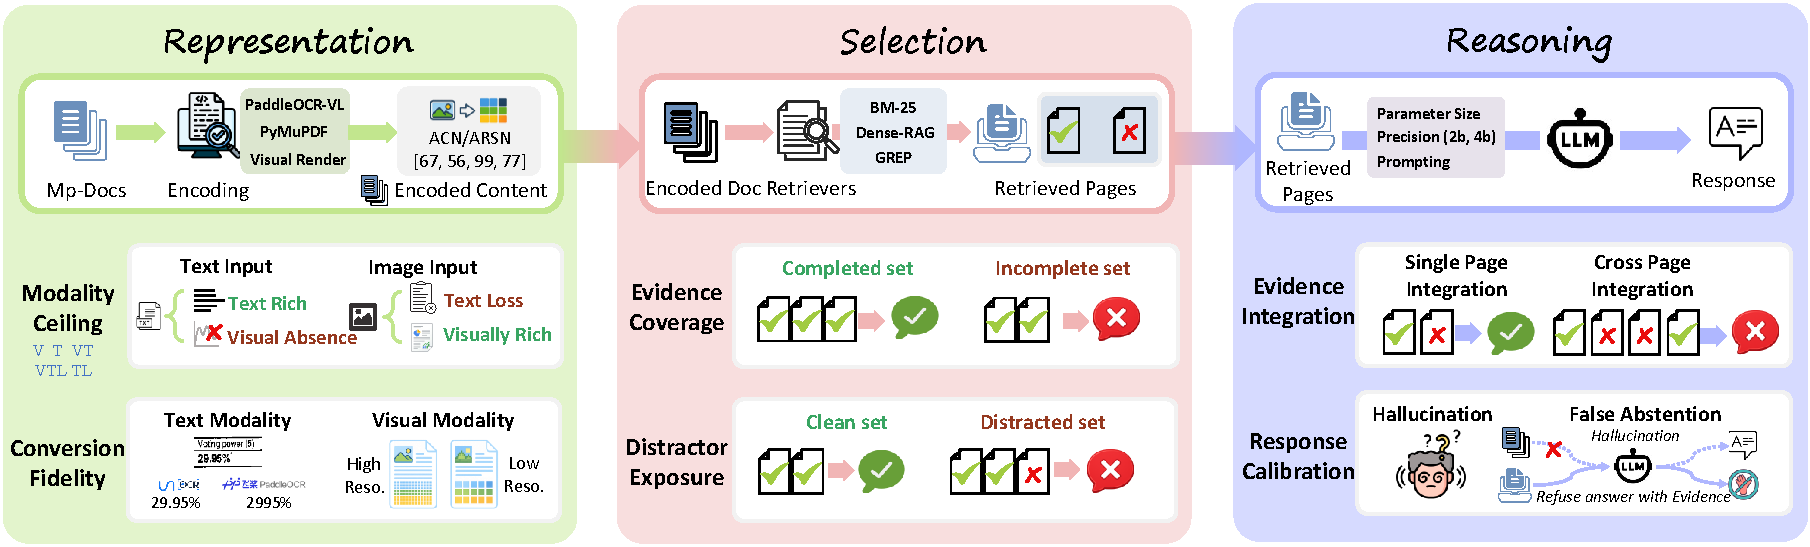
\includegraphics[width=\linewidth]{figures/framework.pdf}
\caption{The three failure loci and six mechanisms informing MP-VRDU design.}
\label{fig:framework}
\end{figure*}

We argue that MP-VRDU design can be decomposed into three fundamental loci defined irrespective of system architecture as \textbf{representation}, \textbf{selection}, and \textbf{reasoning}. All MP-VRDU techniques target failure at one or more of these loci. For example, Retrieval and adaptive reranking primarily address selection, while agentic techniques can span all three: gathering further evidence addresses selection, re-rendering a region addresses representation, and revising an answer addresses reasoning. This decomposition connects architectural choices to the failures they seek to minimize. Figure~\ref{fig:framework} summarises the loci and their associated mechanisms.

\subsection{Representation}
\label{sec:fm_representation}

Representation converts the document into the artifact consumed by later stages, such as embedded text, parser markdown, rendered pages, or visual crops. This locus concerns document conversion, while backbone operations after tokenization, including projection, resampling, and compression, belong to the reasoning loci.
\textbf{(1) Modality Ceiling.} A representation limits which signals are accessible at its available granularity: text may omit non-linguistic visual information, while images require sufficient resolution to expose fine detail.
\textbf{(2) Conversion Fidelity.} Conversion may degrade information that the modality could otherwise preserve, for example through OCR errors or corrupted table structure~\citep{zhang2025ocr}.

\subsection{Selection}
\label{sec:fm_selection}

Selection determines which represented document content is placed before the reasoner within the available context budget. It may operate over pages, sections, tables, or visual crops, in a single pass or through repeated acquisition.
\textbf{(1) Evidence Coverage.} Coverage measures the proportion of required evidence units included in the selected context; omission leaves the reasoner without information needed for the answer.
\textbf{(2) Distractor Exposure.} Exposure measures irrelevant or misleading content accompanying the required evidence, increasing the burden of identifying and using the relevant information even when coverage is complete.

\subsection{Reasoning}
\label{sec:fm_reasoning}

Reasoning maps the supplied evidence and instruction to a response, which may be a final answer, structured output, or an agentic tool call. When representation preserves the required evidence and selection supplies it, remaining failures concern how the reasoner interprets and acts on that evidence. Although such failures take many forms, we focus on two mechanisms particularly relevant to MP-VRDU:
\textbf{(1) Evidence Integration.} The reasoner may process individual evidence units correctly yet fail to combine them across pages or sources; long-context position effects can amplify this difficulty~\citep{liu2024lost}.
\textbf{(2) Response Calibration.} The decision to answer should reflect evidential support: failure includes unsupported answering (hallucination) and false abstention despite sufficient evidence. These opposing outcomes must be assessed jointly because greater willingness to answer can reduce false abstention while increasing unsupported responses~\citep{whitehead2022reliable}.

\section{Methodology}
\label{sec:methodology}

We test the six failure mechanisms through controlled experiments, derive design implications from the results, and validate these implications at the system level. Appendix~\ref{app:full_experimental_detail} provides full experimental specifications.

\subsection{Attribution by Construction}
\label{sec:attribution}

We instantiate the three failure loci in a \textbf{single-pass retriever-generator} document answering pipeline. Its stages align with the framework: \emph{encoding} determines the representation available to the system, \emph{retrieval} determines which pages reach the reasoner, and \emph{inference} determines how the supplied evidence is used to answer. The encoding stage converts each page to parser markdown, a rendered image, or both. The retrieval stage scores pages against the question and selects the top $k$ at page granularity; oracle conditions instead supply annotated gold pages. The inference stage gives a VLM only the selected pages, the question, and a task instruction, then produces an answer in one pass. Because the stages act once and in order, we can construct comparisons that change the representation, page set, or reasoning instruction relevant to a failure mechanism while holding the other stages fixed. This is how we attribute changes in performance to the mechanisms in \S\ref{sec:attribution_framework}.

\subsection{Experiments}
\label{sec:experiment_design}

\paragraph{Representation.}
To test the modality ceiling, we supply gold pages as embedded text extracted by PyMuPDF (\textbf{T}), PaddleOCR-VL markdown (\textbf{TL})~\citep{cui2025paddleocr}, markdown plus page images (\textbf{TLV}), or images alone (\textbf{V}), and compare results by evidence source. To test conversion fidelity, we compare PaddleOCR-VL with MinerU 2.5~\citep{niu2026mineru2} and Unlimited-OCR~\citep{yin2026unlimited} within \textbf{TL} and \textbf{TLV}, then sweep the \texttt{low}, \texttt{med}, and \texttt{high} image presets (see Appendix~\ref{app:representation}) within \textbf{V} and \textbf{TLV}. The parser and resolution changes are evaluated separately. The default is \textbf{TLV} with PaddleOCR-VL and \texttt{med}: pages are rendered at 200 DPI and downsampled to 501,760 pixels per page (a median of 456 visual tokens). 

\paragraph{Selection.}
To test evidence coverage, we start from the complete gold-page set for each multi-page question. ColQwen3, a ColPali-style visual retriever~\citep{faysse2025colpali} is used to rank the document pages, we then remove either the highest- or lowest-ranked gold page, or retain only one of them. To test distractor exposure, we keep the complete gold set and add the highest-ranked non-gold pages. Each condition is compared with its complete-gold baseline on the same questions. We group exposure results by gold-page count, and present all supplied pages in document order.

\paragraph{Reasoning.}
Qwen3-VL-8B-Instruct~\citep{team2025qwen3} runs in \texttt{bf16} with greedy decoding. To test evidence integration, we group answerable questions by evidence-page and evidence-source count, then compare \texttt{none} and chain-of-thought (\texttt{cot}) on matched gold pages. To test calibration, we compare \texttt{none} and \texttt{abstain} on answerable questions with gold pages and unanswerable questions with BM25's top three pages. We also test \texttt{abstain\_cot}, which combines the two instructions. The output limit is 256 tokens, or 2048 for prompts containing CoT.

\paragraph{Validation.}
We test whether the design implications remain useful when combined in the system described in \S\ref{sec:simple_adaptive_method}. Without oracle page selection, we compare its accuracy with a configuration-matched, single-pass gold-page baseline and published systems. We report results by evidence source, page count, and answerability, then analyse remaining errors in evidence acquisition, presentation, integration, and refusal.

% % tables/MMLongBench.tex — MMLongBench-Doc summary + domain breakdown. Single-column, two panels.
%
% The evidence-page rows are ANSWERABLE-ONLY counts, recomputed from the staged parquet
% (.data/mmlongbench/data/train-00000-of-00001.parquet): 1 page 480 · 2 pages 246 ·
% 3+ pages 112, plus 9 answerable questions that carry no annotated gold pages (847 total).
% The 9 are not given a row: they are a corpus quirk, not a finding, and explaining them
% costs more space than they are worth. The sub-rows therefore sum to 838, and the caption
% carries the one clause that accounts for the difference.
%
% Do NOT take these from docs/generated/mmlongbench_stats.md's "Derived hop" table: that
% table is a census of all 1091 questions INCLUDING the unanswerable ones, and 7
% unanswerable questions do carry evidence pages (5 with one page, 1 with two, 1 with six).
% Its 485/247 are therefore corpus-wide, not answerable-only, and exceed the correct
% 480/246 by exactly those.
%
% These counts are the denominators used by tables/Integration.tex (single 480, multi 358
% = 246 + 112, i.e. 838 once the 9 no-gold-page questions are dropped).
\begin{table}[t]
\centering
\small
\setlength{\tabcolsep}{5pt}
\begin{tabular}{lrclr}
\toprule
\multicolumn{2}{c}{\textbf{Summary}} && \multicolumn{2}{c}{\textbf{By domain}} \\
\cmidrule{1-2}\cmidrule{4-5}
\textbf{Property} & \textbf{Value} && \textbf{Domain} & \textbf{Q} \\
\midrule
  Questions          & 1091   && Research report   & 293 \\
  \quad Answerable    & 847    && Academic paper    & 204 \\
  \quad\quad 1 page    & 480    && Guidebook         & 156 \\
  \quad\quad 2 pages   & 246    && Tutorial/Workshop & 139 \\
  \quad\quad 3+ pages  & 112    && Financial report  & 117 \\
  \quad Unanswerable  & 244    && Brochure          & 101 \\
  Mean pages/doc     & 48.3   && Admin/Industry    &  81 \\
  Pages min--max     & 9--468 && Total             & 1091 \\
\bottomrule
\end{tabular}
\caption{MMLongBench-Doc composition.}
% Evidence-page counts are answerable questions only; nine carry no annotated gold pages.}
\label{tab:mmlongbench}
\end{table}


\subsection{Dataset and Evaluation}
\label{sec:dataset_evaluation}

MMLongBench-Doc~\citep{ma2024mmlongbench} contains 135 documents with textual, tabular, graphical, and layout-dependent evidence. Its annotations identify evidence pages, evidence sources, document domains, and unanswerable questions, supporting oracle selection, constructed evidence perturbations, source-specific analysis, and calibration evaluation.

We use Gemini-2.5-Flash at temperature zero to judge answer correctness. The official rule-based scorer can mark semantically correct answers wrong when they differ from the gold answer in units, rounding, or formatting; an LLM judge accommodates these variations across the experimental conditions. It is provided only the question, gold answer, unanswerable flag, and extracted model answer. Accuracy is the proportion judged correct, while paired transitions track correct-to-incorrect and incorrect-to-correct changes on the same questions. A separate analysis rubric identifies abstentions and answer-error categories. Judge agreement is 96.0\% with GPT-4o and 98.3\% with a human annotator on validation subsets. System-level comparisons with published results use the benchmark's official scoring protocol.

\section{Design Implications}
\label{sec:findings}

In this section, we connect failures in representation, selection, and reasoning to design implications for MP-VRDU systems.

\subsection{Representation}
\label{sec:findings_representation}

% GENERATED by ops/scripts/tables/ -- do not edit by hand, re-run the script.
% Numbers read from results/tables/analysis/*.csv.
% analysis/faithfulness_answerable_accuracy_source and analysis/ldu_source_outcomes
% (results.errcat.jsonl)
% Shade ranges are fitted to the values present: abstention neutral over
% [0.7, 36.6], accuracy accteal over [14.5, 78.2]
\definecolor{neutral}{HTML}{5B6B7F}
\definecolor{accteal}{HTML}{1BAF7A}
\begin{table}[t]
\centering
\small
\resizebox{\columnwidth}{!}{%
\setlength{\tabcolsep}{4pt}%
\begin{tabular}{@{}l cccc @{\hskip 10pt} cccc@{}}
\toprule
 & \multicolumn{4}{c}{\textbf{Abstention}} & \multicolumn{4}{c}{\textbf{Accuracy}} \\
\cmidrule(r){2-5}\cmidrule(l){6-9}
\textbf{Evidence} & \textbf{T} & \textbf{TL} & \textbf{TLV} & \textbf{V} & \textbf{T} & \textbf{TL} & \textbf{TLV} & \textbf{V} \\
\midrule
\multicolumn{9}{@{}l}{\textbf{MMLongBench-Doc}} \\
\quad Text & \cellcolor{neutral!37}23.0 & \cellcolor{neutral!18}11.5 & \cellcolor{neutral!11}7.3 & \cellcolor{neutral!12}8.0 & \cellcolor{accteal!21}36.9 & \cellcolor{accteal!28}44.4 & \cellcolor{accteal!34}\textbf{51.0} & \cellcolor{accteal!26}42.3 \\
\quad Layout & \cellcolor{neutral!33}20.3 & \cellcolor{neutral!16}10.2 & \cellcolor{neutral!0}0.8 & \cellcolor{neutral!6}4.2 & \cellcolor{accteal!11}26.3 & \cellcolor{accteal!18}33.9 & \cellcolor{accteal!33}\textbf{49.2} & \cellcolor{accteal!27}43.2 \\
\quad Table & \cellcolor{neutral!25}15.9 & \cellcolor{neutral!11}7.2 & \cellcolor{neutral!10}6.7 & \cellcolor{neutral!14}\textbf{9.1} & \cellcolor{accteal!20}35.6 & \cellcolor{accteal!28}\textbf{44.7} & \cellcolor{accteal!28}\textbf{44.7} & \cellcolor{accteal!18}34.1 \\
\quad Chart & \cellcolor{neutral!53}32.6 & \cellcolor{neutral!46}\textbf{28.1} & \cellcolor{neutral!11}7.3 & \cellcolor{neutral!9}6.2 & \cellcolor{accteal!2}16.3 & \cellcolor{accteal!2}16.9 & \cellcolor{accteal!27}\textbf{42.7} & \cellcolor{accteal!24}40.4 \\
\quad Figure & \cellcolor{neutral!60}\textbf{36.6} & \cellcolor{neutral!40}24.8 & \cellcolor{neutral!12}\textbf{7.6} & \cellcolor{neutral!12}7.9 & \cellcolor{accteal!0}14.5 & \cellcolor{accteal!7}22.1 & \cellcolor{accteal!26}\textbf{42.4} & \cellcolor{accteal!23}39.0 \\
\quad \emph{All} & \cellcolor{neutral!43}26.3 & \cellcolor{neutral!28}17.2 & \cellcolor{neutral!9}6.2 & \cellcolor{neutral!11}7.1 & \cellcolor{accteal!14}29.0 & \cellcolor{accteal!20}35.7 & \cellcolor{accteal!33}\textbf{49.5} & \cellcolor{accteal!26}42.6 \\
\midrule
\multicolumn{9}{@{}l}{\textbf{LongDocURL}} \\
\quad Text & \cellcolor{neutral!7}4.6 & \cellcolor{neutral!5}3.5 & \cellcolor{neutral!1}\textbf{1.5} & \cellcolor{neutral!2}\textbf{1.6} & \cellcolor{accteal!54}71.8 & \cellcolor{accteal!58}75.6 & \cellcolor{accteal!60}\textbf{78.2} & \cellcolor{accteal!52}70.0 \\
\quad Layout & \cellcolor{neutral!2}2.1 & \cellcolor{neutral!2}1.6 & \cellcolor{neutral!0}0.7 & \cellcolor{neutral!0}0.9 & \cellcolor{accteal!29}45.0 & \cellcolor{accteal!33}49.2 & \cellcolor{accteal!35}\textbf{51.3} & \cellcolor{accteal!33}49.3 \\
\quad Table & \cellcolor{neutral!7}5.0 & \cellcolor{neutral!4}3.2 & \cellcolor{neutral!1}1.1 & \cellcolor{neutral!0}0.8 & \cellcolor{accteal!41}57.7 & \cellcolor{accteal!48}\textbf{65.6} & \cellcolor{accteal!46}63.6 & \cellcolor{accteal!36}52.4 \\
\quad Figure & \cellcolor{neutral!10}\textbf{6.7} & \cellcolor{neutral!13}\textbf{8.6} & \cellcolor{neutral!1}\textbf{1.5} & \cellcolor{neutral!1}1.3 & \cellcolor{accteal!43}59.9 & \cellcolor{accteal!45}62.8 & \cellcolor{accteal!52}\textbf{69.9} & \cellcolor{accteal!45}61.9 \\
\quad \emph{All} & \cellcolor{neutral!7}4.7 & \cellcolor{neutral!6}4.3 & \cellcolor{neutral!1}1.3 & \cellcolor{neutral!1}1.3 & \cellcolor{accteal!43}60.3 & \cellcolor{accteal!47}64.5 & \cellcolor{accteal!50}\textbf{67.3} & \cellcolor{accteal!42}59.4 \\
\bottomrule
\end{tabular}%
}
\caption{Abstention and accuracy by evidence source and representation.}
% Shares (\%) of answerable questions with gold pages supplied and no abstention instruction, on MMLongBench-Doc and on LongDocURL: declined, and answered correctly, at each representation. T is embedded text, TL parser text, TLV parser text with page images, V images alone. Bold marks the source declined most in each abstention column and the best representation in each accuracy row. Text-only input leaves chart and figure questions declined most often and page images bring every source under 10\%, and no representation is more accurate than joint input on any source. On LongDocURL, whose documents are born-digital, no source is declined more than one time in ten at any representation and the image adds little to parser text.
\label{tab:abstention_rungs}
\end{table}
% {\footnotesize\raggedright
% Oracle pages, answerable pool, Qwen3-VL-8B bf16, under the error-taxonomy judge, the one that
% defines the abstained verdict. LongDocURL annotates four sources and no charts. A question citing several sources counts under each, so the source rows
% overlap and do not sum to \emph{All}, which pools each question once and is left out of the
% bold contest. At T a scanned page has no text layer, so part of that column is the reasoner
% correctly declining what the rung delivered. The unanswerable pool is absent by construction:
% 235 of its 244 questions carry no evidence-source label.\par}


%\paragraph{Modality Ceiling: Missing Visual Structure Prompts Abstention.}
\paragraph{Modality Ceiling: Pair Text with Vision to Cover Different Evidence.}
With gold pages supplied and no abstention instruction, the reasoner declines chart and figure questions much more often under \textbf{T} and \textbf{TL} than when it receives page images (Table~\ref{tab:abstention_rungs}). Extracted text can preserve labels, captions, and numbers while losing the spatial relationships among graphical elements. Parser markdown recovers some document structure, but cannot reliably express every relationship that a chart or figure encodes. Images make this evidence available and bring abstention below 10\% across evidence sources. Yet \textbf{V} remains less accurate than \textbf{TLV}: seeing the page does not guarantee reliable reading of dense text or precise values at the available resolution. Text and images thus cover different evidential needs, favoring their combination when the questions a system will face are varied.

\begin{figure}[t]
\centering
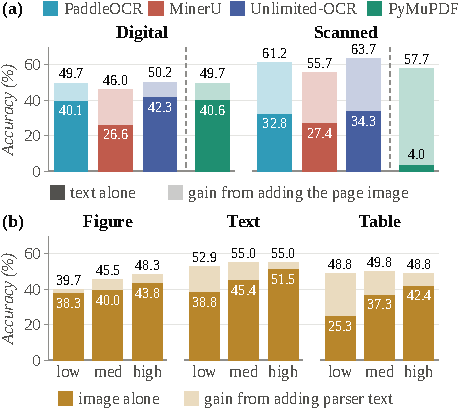
\includegraphics[width=\columnwidth]{figures/fidelity.pdf}
\caption{Conversion fidelity across text and visual channels.}% Top: text-only accuracy and the gain from adding page images, by parser and scan status. Bottom: image-only accuracy and the gain from adding parser text, by image resolution.}
\label{fig:fidelity}
\end{figure}

%\paragraph{Redundant Channels Buffer Conversion Errors.}
\paragraph{Prioritise Conversion Fidelity Where Redundancy Cannot Compensate.}
Conversion errors matter most when the other channel cannot recover the affected evidence, consistent with prior findings on OCR errors~\citep{zhang2025ocr,sun2026when}. On digital documents, the 15.7-point accuracy spread between parsers with text alone contracts to 4.2 points when page images are added (Figure~\ref{fig:fidelity}): the image can preserve content that parsing omits or distorts. Scans expose the same dependence more sharply, since PyMuPDF text reaches only 4.0\% without a usable embedded text layer, while adding the image raises accuracy to 57.7\%. Parser text likewise reduces dependence on image resolution. From \texttt{low} to \texttt{high}, image-only accuracy gains 12.7 points for text questions and 17.1 for table questions, compared with 2.1 and 0.0 points when parser text is present. Figure questions remain sensitive to resolution even with parser text, gaining 8.6 points across the same sweep. Fidelity therefore matters most where the detail cannot be recovered from a complementary channel.

\subsection{Selection}
\label{sec:findings_selection}

\begin{figure}[t]
\centering
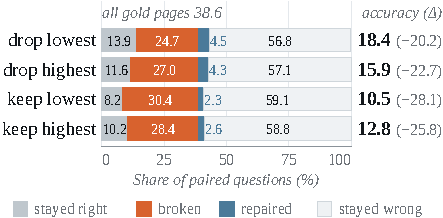
\includegraphics[width=\columnwidth]{figures/coverage.pdf}
\caption{Paired verdict transitions and accuracy after removing or retaining gold pages.}
\label{fig:coverage}
\end{figure}

\paragraph{Prioritize Evidence Coverage.}
MMLongBench-Doc identifies gold pages as the minimal set required to answer each question, so removing one should impair performance. The experiment quantifies this effect: accuracy falls from 38.6\% to 18.4\% when the lowest-ranked gold page is removed and to 15.9\% when the highest-ranked page is removed (Figure~\ref{fig:coverage}). Both losses are substantial, indicating that retrieval rank alone cannot identify which required pages to omit. A practical selector should prioritize evidence coverage, even when some relevant pages rank lower.

\begin{figure}[t]
\centering
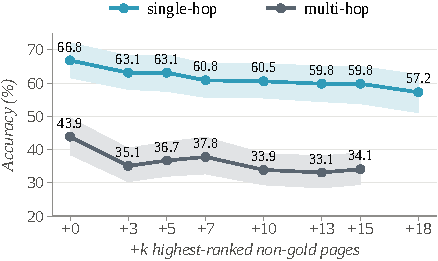
\includegraphics[width=\columnwidth]{figures/distractor_k_hop.pdf}
\caption{Accuracy and paired verdict transitions as non-gold pages are added to complete gold-page sets.}% Single-hop questions require one page and one evidence source; all other questions are classified as multi-hop.}
\label{fig:distractor_k}
\end{figure}

\paragraph{Distractor Exposure: Acquire Broadly, Present Selectively.}
Adding non-gold pages leaves the required evidence available but makes it harder to identify and use. With three added pages, accuracy falls from 66.8\% to 63.1\% for single-hop questions and from 43.9\% to 35.1\% for multi-hop questions (Figure~\ref{fig:distractor_k}). Questions spanning multiple pages or evidence sources may be more vulnerable because plausible context can interfere with selecting and combining the required facts. Some answers improve, however, suggesting that pages outside the annotations can clarify the gold evidence. Broader acquisition can thus recover useful context, but the pages presented to the reasoner should be selected to limit competing or misleading evidence.

\subsection{Reasoning}
\label{sec:findings_reasoning}

\begin{figure}[t]
\centering
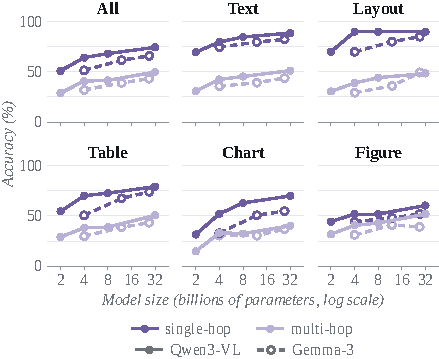
\includegraphics[width=\columnwidth]{figures/reasoning_combined.pdf}
\caption{Response outcomes under the \texttt{none}, \texttt{cot}, and \texttt{abstain} prompts.}
\label{fig:reasoning_combined}
\end{figure}

\paragraph{Match Reasoning to Evidence Structure and Sufficiency.}
Intermediate reasoning is useful when it has evidence to connect. With the same gold pages supplied, CoT lowers single-hop accuracy from 63.4\% to 59.7\% but raises multi-hop accuracy from 38.5\% to 43.3\% (Figure~\ref{fig:reasoning_combined}). For a direct answer, extra steps can introduce errors; for distributed evidence, they can help maintain the relationships needed to answer. CoT does not resolve the separate question of whether the evidence is sufficient: unanswerable refusal remains near the uninstructed rate. The \texttt{abstain} instruction raises that refusal to 74.6\%, but also produces false refusals on answerable questions, especially multi-hop ones. Evidence that takes work to assemble can appear absent under a general instruction to be cautious. The resulting design principle is to use intermediate reasoning for integration and to make refusal depend on identifying missing facts.

\begin{figure}[t]
\centering
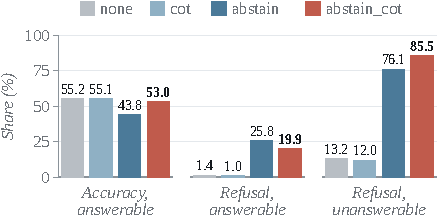
\includegraphics[width=\columnwidth]{figures/abstain_cot_bars.pdf}
\caption{Answerable accuracy and unanswerable refusal across the four prompt modes. \texttt{abstain\_cot} combines the CoT and abstention instructions.}
\label{fig:reasoning_abstain_cot}
\end{figure}

\paragraph{Reason Through the Evidence Before Deciding to Abstain.}
The combined \texttt{abstain\_cot} prompt suggests how to put these two instructions in a useful order. It raises unanswerable refusal from 76.1\% under \texttt{abstain} to 85.5\%, while recovering answerable accuracy from 43.8\% to 53.0\%, near the uninstructed 55.2\% (Figure~\ref{fig:reasoning_abstain_cot}). Qwen3-VL-8B-Instruct has vision--language training that includes multi-page document question answering, although it is the non-thinking variant post-trained on standard instruction formats rather than the Thinking variant's CoT-formatted responses~\citep{team2025qwen3}. The prompt may therefore direct an existing capability: assemble what the pages establish before deciding whether the abstention rule applies. The comparison does not reveal the model's internal process, but it motivates a system design that checks the question's premises against accumulated evidence before either answering or refusing.

\section{System-level Validation}
\label{sec:simple_adaptive_method}

We combine the preceding design implications in a deliberately simple adaptive system. Where suitable, it borrows familiar mechanisms from existing pipelines, such as iterative reading into an evidence memory~\citep{jain2025simpledoc} and answer verification~\citep{zhu2026doclens}. We then test whether this combination achieves competitive performance compared to other published methods using the same backbone.

\subsection{Validation System Design}
\label{sec:system_design}

\begin{figure}[t]
\centering
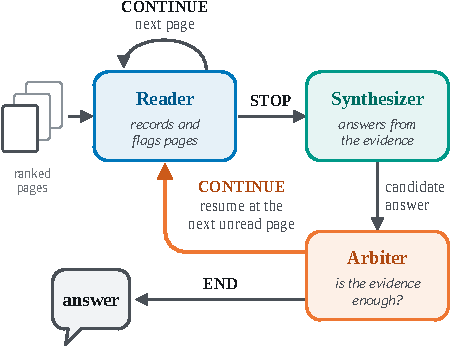
\includegraphics[width=\columnwidth]{figures/simple_method_column.pdf}
\caption{Architecture of our validation system.}
\label{fig:simple_method_arch}
\end{figure}

Three roles share one vision-language model but receive different instructions and evidence (Figure~\ref{fig:simple_method_arch}). The \texttt{reader} visits pages in retrieval-ranked order to encounter likely relevant evidence early. At each turn, it records the page's contribution in a persistent evidence memory and flags pages that the \texttt{synthesizer} may need to inspect in full. After a minimum reading depth, the \texttt{reader} may stop. The \texttt{synthesizer} then receives the memory and flagged pages in full \textbf{TLV} and constructs a candidate answer. The \texttt{arbiter} checks whether the gathered evidence is sufficient to support that answer; it either accepts the candidate or resumes reading at the next unread page. This cycle continues until the answer is accepted or the page budget is reached. Retrieval determines the visiting order, so the same architecture could instead traverse pages in document order. Appendix~\ref{app:val_system_details} provides full implementation details.

\paragraph{Representation.}
When a page is presented in full, parser text accompanies its image because the two channels preserve different kinds of evidence. This pairing resembles pipelines that process text and vision together~\citep{han2025mdocagent}. Unlimited-OCR, the strongest parser in our comparison, supplies the text channel. The \texttt{reader} also receives high-resolution images to preserve fine visual detail where parsing may be insufficient.

\paragraph{Selection.}
The system acquires evidence broadly but presents it selectively. Since omitting a required page is more damaging than inspecting an additional page, the \texttt{reader} must reach a minimum reading depth before stopping. On each turn, it records what the current page contributes toward answering the question, building an evidence memory that persists across reading turns. It also flags pages that may need to be examined in full, including when their relevance is uncertain. Flagged pages reach the \texttt{synthesizer} in full \textbf{TLV}; other inspected pages contribute only their records. This resembles SimpleDoc's iterative evidence memory~\citep{jain2025simpledoc}, while selective full-page presentation addresses our distractor findings.

\paragraph{Reasoning.}
The \texttt{synthesizer} reasons step by step over the accumulated evidence, allowing it to combine facts across pages when the question requires integration. It checks the question's premises and must name a specific missing fact before returning \emph{Not answerable}. The \texttt{arbiter} then checks the candidate against the flagged pages, a verification step related to DocLens's answer adjudication~\citep{zhu2026doclens}. It cannot replace the answer: it either accepts it or identifies a missing fact and resumes reading from the next unread page. This gives an apparent evidence gap a chance to be resolved through acquisition before refusal becomes final. A page budget bounds the cycle.

% The system uses complementary text and visual channels to address representation loss, broad acquisition and selective presentation to balance evidence coverage with distractor exposure, and structured synthesis and sufficiency checking to address integration and calibration. Three roles, implemented by the same vision-language model, carry out these steps: a \texttt{reader}, a \texttt{synthesizer}, and an \texttt{arbiter}.

% \paragraph{(1) Reader: Acquire Evidence Selectively.}
% The \texttt{reader} traverses pages in retrieval-ranked order using joint textual and visual input. It records answer-relevant evidence from each page and flags pages it judges necessary to present to the \texttt{synthesizer} in full \textbf{TLV}. Because omitting a required page is more damaging than inspecting an additional non-gold page, the \texttt{reader} flags pages when relevance is uncertain. Records from unflagged pages remain available as context without adding every inspected page to the final multimodal input. Once the minimum reading depth is reached, the \texttt{reader} may propose \texttt{STOP} when it considers the collected evidence sufficient.

% \paragraph{(2) Synthesizer: Integrate Evidence and Check Premises.}
% The \texttt{synthesizer} receives evidence in document order: flagged pages in full \textbf{TLV} and compact records from other pages. When no page is flagged, the two highest-ranked inspected pages provide fallback context. Full pages let it verify details that a reader record may omit or misstate, while records preserve context gathered during broader acquisition. The \texttt{synthesizer} combines CoT reasoning, which helped on multi-hop questions, with premise checking and an abstention instruction. It must test the details assumed by the question rather than answer from a nearby match; before returning \emph{Not answerable}, it must identify the specific missing fact.

% \paragraph{(3) Arbiter: Check Sufficiency and Resume Acquisition.}
% The \texttt{arbiter} receives the accumulated records, flagged pages in full \textbf{TLV}, and the \texttt{synthesizer}'s candidate answer. Seeing the evidence pages that produced the answer lets it assess support against the source evidence, including details a record may have missed. It either accepts the answer or names a missing fact and requests further reading; it cannot replace the answer itself. On \texttt{CONTINUE}, the \texttt{reader} resumes at the next unread page before another synthesis turn. This gives an apparent evidence gap a chance to be resolved through acquisition, addressing the observed tendency of abstention prompts to refuse answerable questions. The page budget bounds the cycle.

\subsection{System Configuration}

\paragraph{Deployment Parameters.}
Five parameters bound the trajectory. $B$ caps the total pages read, $p$ sets pages read per reader turn, $k$ is the minimum number of initial \texttt{reader} turns before a \texttt{STOP} is honoured, and $m$ is the minimum number of additional turns after reading resumes from an arbiter \texttt{CONTINUE} decision. We choose these parameters specifically to run on a single NVIDIA V100 16\,GB GPU and to guard against premature stopping, with $B=30$, $p=1$, $k=6$, and $m=4$.

\paragraph{Configuration.}
All three roles share \texttt{Qwen3-VL-8B-Instruct} with 4-bit NF4 quantization, FP16 compute, and greedy decoding. ColQwen3.5 ranks pages once per question. The \texttt{reader} receives Unlimited-OCR text and high-resolution page images; flagged pages shown to the \texttt{synthesizer} and \texttt{arbiter} use the same text with medium-resolution images. We evaluate MMLongBench-Doc with its official scoring protocol and report accuracy by evidence source, page count, and answerability, together with acquisition depth, role invocations, token use, latency, and peak GPU memory. The LongDocURL evaluation is pending. Appendix~\ref{app:setup_details} includes full prompts and implementation details.

\subsection{Validation Outcomes}
\label{sec:simple_method_results}

% Hand-maintained (not generated): the official-protocol rows of
% tables/include/simple_method_results_v2.tex and tables/include/ldu_method_results.tex in
% one table, a row per system, without MMLongBench-Doc's evidence-source columns. Method
% names carry no citation; cite them where the baselines are introduced:
%   MDocAgent han2025mdocagent, M3DocRAG cho2024m3docrag, MoLoRAG wu2025molorag,
%   DocAgent sun2025docagent, MARDoc chen2026mardoc, DocTrace xiang2026doctrace,
%   SLEUTH liu2025resolving.
% Qwen3-VL-8B rows only; the Qwen2.5-VL-7B block is in tables/paper/method_results.tex.
% Ours on MMLongBench-Doc is iteration 7's official-protocol block in
% results/method/results_v7.md (1,067 of the 1,082 questions finished). The LongDocURL
% numbers for Ours and for the gold-pages row are from results/method/ldu_official.md
% (`python -m seqread.official_ldu`). PROVISIONAL: Ours is on the 583 of 1,002 subset
% questions finished so far; refresh it, and drop footnote d, when the run is complete.
\begin{table*}[t]
\centering
\small
\newcommand{\yes}{\checkmark}
\newcommand{\no}{$\times$}
\resizebox{\textwidth}{!}{%
\setlength{\tabcolsep}{7pt}%
\begin{tabular}{@{}lcc cccc cccc@{}}
\toprule
& & & \multicolumn{4}{c}{\textbf{MMLongBench-Doc}} & \multicolumn{4}{c}{\textbf{LongDocURL}} \\
\cmidrule(lr){4-7}\cmidrule(l){8-11}
\textbf{Method} & \textbf{OCR} & \textbf{Trained}
& SIN & MUL & UNA & \textbf{ACC} & UND & REA & LOC & \textbf{ACC} \\
\midrule
Gold pages + VLM & \yes & \no & 57.7 & 37.4 & 52.5 & 49.5 & 69.7 & 63.6 & 59.5 & 65.7 \\
\addlinespace
Whole document (via DocTrace) & \no & \no & 46.9 & 35.3 & 25.8 & 38.5 & -- & -- & -- & 45.1 \\
M3DocRAG (via SLEUTH) & \no & \no & -- & -- & 48.6 & 45.9$^{a}$ & 60.1 & 52.4 & 45.5 & 54.6 \\
DocAgent (via MARDoc) & \yes & \no & -- & -- & -- & 46.6 & -- & -- & -- & -- \\
MDocAgent (via SLEUTH) & \yes & \no & -- & -- & 49.7 & 47.8$^{a}$ & 57.5 & 51.5 & 44.7 & 53.1 \\
MoLoRAG (via SLEUTH) & \no & \no & -- & -- & 51.7 & 48.8$^{a}$ & 63.4 & 52.7 & 49.3 & 57.6 \\
% MARDoc & \yes & \no$^{b}$ & -- & -- & -- & 52.7 & -- & -- & -- & -- \\
SLEUTH & \no & \no & -- & -- & 67.4 & 52.8$^{a}$ & 65.7 & 53.0 & \textbf{53.6} & 60.0 \\
DocTrace & \yes & \yes & 53.2 & \textbf{41.1} & 70.5 & 52.9 & -- & -- & -- & 56.4 \\
\textbf{Ours} (4-bit) & \yes & \no & \textbf{60.5} & 39.2 & \textbf{76.9} & \textbf{56.5} & \textbf{66.4}$^{d}$ & \textbf{63.6}$^{d}$ & 51.2$^{d}$ & \textbf{61.3}$^{d}$ \\
\bottomrule
\end{tabular}%
}
\caption{\small Accuracy (\%) under each benchmark's official protocol. Every system we compare against uses Qwen3-VL-8B as its backbone, as ours does. ``via'' marks a result reproduced by another study, and ``--'' indicates not reported. \textbf{OCR}: parser or OCR text is an input. \textbf{Trained}: task-specific fine-tuning or RL in the pipeline. $^{a}$The average SLEUTH reports over its evidence-type columns, which is not accuracy over all questions.}
\label{tab:method_results}
\end{table*}


% \paragraph{Performance on MMLongBench-Doc.}
% The system reaches 56.5\% official-protocol accuracy, the highest reported overall score among the open 7--8B systems in Table~\ref{tab:mmlb_method_results}. It exceeds the reported DocTrace and MARDoc scores by 3.6 and 3.8 points, respectively, though differences in evaluation setups may account for some of this gap. Performance is strongest on tables (62.1\%) and weaker on layout (43.0\%), charts (41.4\%), and figures (41.4\%). Text and table details can often be preserved in parser output and reader records, whereas spatial relationships and graphical features are harder to carry through a compact record when a page is not flagged for full presentation. The 39.2\% multi-page accuracy, below DocTrace's 41.1\%, also shows that supplying selected pages does not resolve every integration failure. These results support the combined design while leaving both visual evidence use and cross-page reasoning as limitations.


\section{Conclusion}
\label{sec:conclusion}

We attributed MP-VRDU failure to representation, selection, and reasoning through controlled interventions, and showed that a deliberately simple system built from the resulting design implications is competitive with an untrained, 4-bit 8B model on a single 16\,GB GPU. Because these implications concern failure loci rather than architectures, existing and future systems can adopt them independently of their design: an iterative reader such as SimpleDoc could present only flagged pages in full, and a verifier such as DocLens's adjudicator could resume acquisition rather than refuse. Testing this transfer is a natural next step. Cross-page integration and the use of visual evidence remain the largest open failures, and resolving them likely requires training rather than prompting alone. Extending attribution to finer evidence granularity, broader model families, and agentic systems would further test how far these implications generalise.

\clearpage
\section*{Limitations}

% \section*{Acknowledgments}

% Bibliography entries for the entire Anthology, followed by custom entries
%\bibliography{anthology,custom}
% Custom bibliography entries only
\bibliography{custom_survey, custom_empirical}

\appendix

\clearpage
% Columns end where their content does, instead of stretching to the page bottom.
\raggedbottom
\section{Additional Experimental Details}
\label{app:full_experimental_detail}

This appendix supplements \S\ref{sec:methodology} with the prompts, settings and evaluation rubrics that the main text does not give.

%% ---------------------------------------------------------------------------
\subsection{Pipeline}
\label{app:attribution}

\begin{figure}[t]
\centering
\begin{tcolorbox}[
  colback=gray!5,
  colframe=gray!50,
  boxrule=0.4pt,
  fontupper=\small\ttfamily,
  left=5pt,right=5pt
]
You are answering a question about a document.\\[0.4em]
\{instruction\}\\[0.4em]
Question:\\
\{question\}\\[0.4em]
Document evidence:\\
\{context\}\\[0.4em]
Answer:
\end{tcolorbox}
\caption{Common single-pass reasoner template. The instruction comes from Table~\ref{tab:app_reasoning_prompts}; the context contains the selected pages in document order and in the representation specified by the condition.}
\label{fig:app_reasoner_template}
\end{figure}

The pipeline of \S\ref{sec:attribution} has three stages, each run once per question.

\paragraph{(1) Encoding.}
Each page is rasterised at 200\,DPI, and its embedded text layer is extracted with PyMuPDF. A document parser converts the rendered page to markdown, one page at a time, and the result is stored so that every condition reads the same parse. Page images are downsampled to the pixel cap of the resolution preset before they reach the reasoner. The representation then determines which of these artifacts form the context (Table~\ref{tab:app_representations}).

\paragraph{(2) Retrieval.}
A retriever scores every page of the question's document against the question and returns the top $k$ pages. Text retrievers rank page text and visual retrievers rank page images. The controlled experiments replace this stage with constructed page sets: representation and reasoning conditions supply the annotated gold pages, and selection conditions remove gold pages or add non-gold ones. ColQwen3 is used only to order pages where a condition depends on rank, and BM25 only to supply three pages for unanswerable questions, which have no gold evidence.

\paragraph{(3) Inference.}
The reasoner receives the selected pages, the question and an instruction in the template of Figure~\ref{fig:app_reasoner_template}, and answers in a single pass without tools or follow-up turns. Pages are restored to document order, whatever their rank. Under \textbf{TLV}, the text of all supplied pages forms one block, followed by their images in the same order. Decoding is greedy, with no sampling parameters and no cap on input tokens, so an output is determined by its question, page set, representation, reasoner, resolution and prompt mode.

\paragraph{Comparisons.}
Every intervention is compared with its baseline on the same questions, and a question that cannot satisfy a condition is excluded from that comparison. A \emph{single-hop} question has one gold page and cites one evidence source; every other answerable question is \emph{multi-hop}.

%% ---------------------------------------------------------------------------
\subsection{Representation Settings}
\label{app:representation}

\begin{table}[t]
\centering
\small
\setlength{\tabcolsep}{4pt}
\renewcommand{\arraystretch}{1.15}
\begin{tabular}{@{}l
  >{\raggedright\arraybackslash}p{\dimexpr 0.50\columnwidth-6pt\relax}
  >{\raggedright\arraybackslash}p{\dimexpr 0.36\columnwidth-6pt\relax}@{}}
\toprule
\textbf{Rep.} & \textbf{Text channel} & \textbf{Image channel} \\
\midrule
T   & PyMuPDF embedded text (no parsing) & -- \\
TL  & PaddleOCR-VL markdown              & -- \\
TV  & PyMuPDF embedded text (no parsing) & Page image (\texttt{med}) \\
TLV & PaddleOCR-VL markdown              & Page image (\texttt{med}) \\
V   & --                                 & Page image (\texttt{med}) \\
\bottomrule
\end{tabular}
\caption{Page representations.}
\label{tab:app_representations}
\end{table}
\begin{table}[t]
\centering
\small
\setlength{\tabcolsep}{4pt}
\renewcommand{\arraystretch}{1.15}
\begin{tabular*}{\columnwidth}{@{\extracolsep{\fill}}l l r@{}}
\toprule
\textbf{Channel} & \textbf{Setting} & \textbf{Detail} \\
\midrule
Text  & PaddleOCR-VL (default) & 0.9B \\
Text  & MinerU 2.5             & 1.2B \\
Text  & Unlimited-OCR          & 3.3B \\
\midrule
Image & \texttt{low}           & 285 tok/page \\
Image & \texttt{med} (default) & 456 tok/page \\
Image & \texttt{high}          & 744 tok/page \\
\bottomrule
\end{tabular*}
\caption{Conversion-fidelity settings.}
\label{tab:app_fidelity}
\end{table}

Table~\ref{tab:app_representations} defines the representations and Table~\ref{tab:app_fidelity} the fidelity settings. Parsers emit page-level markdown, and no layout coordinates reach the reasoner. \textbf{T} reads the PDF's embedded text layer, which is usually empty on scanned documents. The image presets cap a page at 313,600 (\texttt{low}), 501,760 (\texttt{med}) and 752,640 (\texttt{high}) pixels, and the token counts in Table~\ref{tab:app_fidelity} are Qwen3-VL's median visual tokens per page.

%% ---------------------------------------------------------------------------
\subsection{Prompt Modes}
\label{app:reasoning}

\begin{table}[t]
\centering
\small
\setlength{\tabcolsep}{4pt}
\renewcommand{\arraystretch}{1.15}
\begin{tabular}{@{}
  >{\raggedright\arraybackslash}p{\dimexpr 0.42\columnwidth-4pt\relax}
  >{\raggedright\arraybackslash}p{\dimexpr 0.58\columnwidth-4pt\relax}@{}}
\toprule
\textbf{Mode} & \textbf{Instruction} \\
\midrule
\texttt{none} & (empty) \\
\texttt{grounded} & Use only the provided document evidence and keep the answer concise. \\
\texttt{abstain} & \texttt{grounded}, plus: If the evidence does not contain the answer, answer exactly: Not answerable. \\
\texttt{abstain\_balanced} & \texttt{abstain}, plus: If the evidence does contain the answer, give it: do not decline a question the evidence supports. \\
\texttt{cot} & \texttt{grounded}, plus: Think step by step before answering. Then write your final answer on a new line beginning with `Answer:'. \\
\texttt{extract\_cot} & \texttt{grounded}, plus a verbatim-evidence extraction step, with visual evidence described in enough detail to answer from the description alone, then reasoning constrained to what was extracted, then the \texttt{Answer:} line. \\
\texttt{abstain\_cot} & \texttt{grounded}, plus: If the evidence does not contain the answer, answer exactly: Not answerable. Think step by step before answering. Then write your final answer on a new line beginning with `Answer:'. \\
\bottomrule
\end{tabular}
\caption{Reasoning prompt modes.}
\label{tab:app_reasoning_prompts}
\end{table}

Table~\ref{tab:app_reasoning_prompts} gives the instruction for each prompt mode, including three that appear only in Appendix~\ref{app:additional_results}. Both \texttt{cot} and \texttt{abstain} include the \texttt{grounded} sentence. Under the modes that request reasoning, the text after the last \texttt{Answer:} marker is extracted as the answer before judging.

%% ---------------------------------------------------------------------------
\subsection{Datasets}
\label{app:datasets_evaluation}

% tables/MMLongBench.tex — MMLongBench-Doc summary + domain breakdown. Single-column, two panels.
%
% The evidence-page rows are ANSWERABLE-ONLY counts, recomputed from the staged parquet
% (.data/mmlongbench/data/train-00000-of-00001.parquet): 1 page 480 · 2 pages 246 ·
% 3+ pages 112, plus 9 answerable questions that carry no annotated gold pages (847 total).
% The 9 are not given a row: they are a corpus quirk, not a finding, and explaining them
% costs more space than they are worth. The sub-rows therefore sum to 838, and the caption
% carries the one clause that accounts for the difference.
%
% Do NOT take these from docs/generated/mmlongbench_stats.md's "Derived hop" table: that
% table is a census of all 1091 questions INCLUDING the unanswerable ones, and 7
% unanswerable questions do carry evidence pages (5 with one page, 1 with two, 1 with six).
% Its 485/247 are therefore corpus-wide, not answerable-only, and exceed the correct
% 480/246 by exactly those.
%
% These counts are the denominators used by tables/Integration.tex (single 480, multi 358
% = 246 + 112, i.e. 838 once the 9 no-gold-page questions are dropped).
\begin{table}[t]
\centering
\small
\setlength{\tabcolsep}{5pt}
\begin{tabular}{lrclr}
\toprule
\multicolumn{2}{c}{\textbf{Summary}} && \multicolumn{2}{c}{\textbf{By domain}} \\
\cmidrule{1-2}\cmidrule{4-5}
\textbf{Property} & \textbf{Value} && \textbf{Domain} & \textbf{Q} \\
\midrule
  Questions          & 1091   && Research report   & 293 \\
  \quad Answerable    & 847    && Academic paper    & 204 \\
  \quad\quad 1 page    & 480    && Guidebook         & 156 \\
  \quad\quad 2 pages   & 246    && Tutorial/Workshop & 139 \\
  \quad\quad 3+ pages  & 112    && Financial report  & 117 \\
  \quad Unanswerable  & 244    && Brochure          & 101 \\
  Mean pages/doc     & 48.3   && Admin/Industry    &  81 \\
  Pages min--max     & 9--468 && Total             & 1091 \\
\bottomrule
\end{tabular}
\caption{MMLongBench-Doc composition.}
% Evidence-page counts are answerable questions only; nine carry no annotated gold pages.}
\label{tab:mmlb_composition}
\end{table}

\begin{table}[t]
\centering
\small
\setlength{\tabcolsep}{5pt}
\renewcommand{\arraystretch}{1.1}
\begin{tabular*}{\columnwidth}{@{\extracolsep{\fill}}lr lr@{}}
\toprule
\textbf{Property} & \textbf{Value} & \textbf{Evidence source} & \textbf{Q} \\
\midrule
Questions        & 2,325   & Text   & 994 \\
Documents        & 396     & Table  & 871 \\
Mean pages/doc   & 85.6    & Layout & 779 \\
Median pages/doc & 78      & Figure & 548 \\
Pages min--max   & 51--149 & Others & 8   \\
\bottomrule
\end{tabular*}
\caption{LongDocURL composition.}
\label{tab:ldu_composition}
\end{table}

Tables~\ref{tab:mmlb_composition} and~\ref{tab:ldu_composition} summarise the two benchmarks. On MMLongBench-Doc, a question is unanswerable when its gold answer is \emph{Not answerable}, and a document is considered scanned when its pages carry no usable text layer. Evidence source is multi-label on both benchmarks, so a question citing two sources counts under both and source counts exceed the number of questions. LongDocURL's documents are born-digital.

%% ---------------------------------------------------------------------------
\subsection{Evaluation}
\label{app:evaluation}

\begin{figure}[t]
\centering
\begin{tcolorbox}[colback=gray!5,colframe=gray!50,boxrule=0.4pt,fontupper=\small\ttfamily,left=5pt,right=5pt]
You judge answers to document questions.\\
Return only JSON with keys:\\
- verdict: one of correct, incorrect, abstained\\
- extracted\_answer: the answer extracted from the model response, or empty string\\
- rationale: a short reason\\[0.5em]
Mark correct when the model answer is semantically equivalent to the gold answer.\\
For unanswerable questions, mark correct only when the model abstains.
\end{tcolorbox}
\caption{Accuracy rubric.}
\label{fig:app_judge_prompt}
\end{figure}

\begin{figure}[t]
\centering
\begin{tcolorbox}[colback=gray!5,colframe=gray!50,boxrule=0.4pt,fontupper=\small\ttfamily,left=5pt,right=5pt]
$\langle$accuracy rubric, with an error\_category key in place of rationale$\rangle$\\[0.5em]
ABSTENTION\\
Return the verdict "abstained" whenever the response declines to answer because it judges the evidence insufficient, however it is worded. "Not answerable", "the document does not provide this", "there is no document evidence to determine this" and "it is not possible to determine this from the given information" are all abstentions. A response that notes a limitation and then commits to an answer anyway is NOT an abstention: judge the answer it commits to.\\[0.5em]
ERROR CATEGORY\\
Decide the verdict FIRST, using only the two rules above, and do not revisit it. The error category explains a verdict you have already reached; it never changes one. In particular, a response that states the gold answer in its own words, or surrounds it with explanation, is still correct.\\[0.5em]
$\langle$the eleven categories of Table~\ref{tab:app_error_taxonomy}, in priority order$\rangle$
\end{tcolorbox}
\caption{Taxonomy rubric.}
\label{fig:app_judge_prompt_taxonomy}
\end{figure}

\begin{table}[t]
\centering
\small
\setlength{\tabcolsep}{4pt}
\renewcommand{\arraystretch}{1.15}
\begin{tabular}{@{}
  >{\raggedright\arraybackslash}p{\dimexpr 0.58\columnwidth-4pt\relax}
  >{\raggedright\arraybackslash}p{\dimexpr 0.42\columnwidth-4pt\relax}@{}}
\toprule
\textbf{Category} & \textbf{Assigned when} \\
\midrule
{\footnotesize\ttfamily insufficient\_evidence} & The response declines: the evidence does not support an answer. \\
{\footnotesize\ttfamily no\_answer\_reached} & It reasons but never commits, trailing off or stopping mid-calculation. \\
{\footnotesize\ttfamily answered\_unanswerable} & The question is unanswerable and a substantive answer is given. \\
{\footnotesize\ttfamily equivocal} & The gold answer is present but not committed to. \\
{\footnotesize\ttfamily wrong\_count} & A ``how many'' question is answered with a different count. \\
{\footnotesize\ttfamily wrong\_value} & A non-count numeric answer differs from the gold value. \\
{\footnotesize\ttfamily wrong\_entity} & A non-numeric answer names a different thing. \\
{\footnotesize\ttfamily incomplete\_list} & The gold answer is a set and the response gives a subset. \\
{\footnotesize\ttfamily over\_inclusive\_list} & The response includes items the gold answer does not. \\
{\footnotesize\ttfamily unit\_or\_format\_mismatch} & The same quantity in a non-matching unit, scale or granularity. \\
{\footnotesize\ttfamily other} & None of the above. \\
\bottomrule
\end{tabular}
\caption{Error categories of the taxonomy rubric, in priority order.}
\label{tab:app_error_taxonomy}
\end{table}

\begin{table}[t]
\centering
\small
\setlength{\tabcolsep}{4pt}
\renewcommand{\arraystretch}{1.15}
\begin{tabular*}{\columnwidth}{@{\extracolsep{\fill}}l r r l@{}}
\toprule
\textbf{Reference} & \textbf{$n$} & \textbf{Agree.} & \textbf{Cohen's $\kappa$ [95\% CI]} \\
\midrule
GPT-4o          & 500 & 96.0\% & 0.918 [0.881, 0.951] \\
Human annotator & 120 & 98.3\% & 0.966 [0.915, 1.000] \\
\bottomrule
\end{tabular*}
\caption{Judge agreement with Gemini-2.5-Flash.}
\label{tab:app_judge_agreement}
\end{table}

\paragraph{Rubrics.}
Gemini-2.5-Flash judges every response under one of two rubrics, the first returning \emph{correct} or \emph{incorrect} only, while the second allows for an additional \emph{abstained} outcome. The \emph{accuracy rubric} (Figure~\ref{fig:app_judge_prompt}) states only the correctness rule. The \emph{taxonomy rubric} (Figure~\ref{fig:app_judge_prompt_taxonomy}) adds a definition of abstention and assigns each incorrect response the first category of Table~\ref{tab:app_error_taxonomy} that applies. Because it recognises refusals however they are worded, it reports more refusals, and its answerable accuracy is two to three points lower. Levels are therefore compared only within a rubric. The taxonomy rubric scores Tables~\ref{tab:abstention_rungs}, \ref{tab:deploy_rungs} and~\ref{tab:app_prompt_results} and Figures~\ref{fig:app_reasoning_cot}--\ref{fig:app_error_sources}; every other result uses the accuracy rubric.

\paragraph{Metrics.}
On unanswerable questions an abstention is correct. On answerable questions it is incorrect and counts as a false refusal. Refusal rates are computed separately for the two pools.

\paragraph{Judge Validation.}
Table~\ref{tab:app_judge_agreement} reports agreement with two references. On 500 stratified responses, Gemini-2.5-Flash agrees with GPT-4o on 96.0\% of verdicts (Cohen's $\kappa = 0.918$), and on a 120-response subset it agrees with a human annotator on 98.3\% ($\kappa = 0.966$).

\clearpage
\section{Additional Results}
\label{app:additional_results}

This appendix extends the results of \S\ref{sec:findings}--\S\ref{sec:deployment}. Unless stated otherwise, results use Qwen3-VL-8B at \textbf{TLV} with gold pages on MMLongBench-Doc.

% The floats of B.1 to B.3 are declared here, ahead of their text and in the order of the
% subsections (representation, selection, reasoning), so they sit at the tops of text pages.
% GENERATED by ops/scripts/tables/ -- do not edit by hand, re-run the script.
% Numbers read from results/tables/mmlongbench/parser_scan_source.csv.
\definecolor{accteal}{HTML}{1BAF7A}
\begin{table}[t]
\centering
\small
\adjustbox{max width=\columnwidth}{%
\setlength{\tabcolsep}{6pt}%
\begin{tabular}{@{}l rr rr@{}}
\toprule
 & \multicolumn{2}{c}{\textbf{Born-digital}} & \multicolumn{2}{c}{\textbf{Scanned}} \\
\cmidrule(lr){2-3}\cmidrule(l){4-5}
\textbf{Text source} & \textbf{Text} & \textbf{+Image} & \textbf{Text} & \textbf{+Image} \\
\midrule
\multicolumn{5}{@{}l}{\emph{PaddleOCR-VL}} \\
\quad Text & \cellcolor{accteal!42}50.9 & \cellcolor{accteal!46}54.9 & \cellcolor{accteal!30}35.4 & \cellcolor{accteal!46}55.4 \\
\quad Layout & \cellcolor{accteal!37}43.8 & \cellcolor{accteal!40}47.5 & \cellcolor{accteal!22}26.3 & \cellcolor{accteal!48}57.9 \\
\quad Table & \cellcolor{accteal!40}47.6 & \cellcolor{accteal!39}46.5 & \cellcolor{accteal!50}59.4 & \cellcolor{accteal!60}71.9 \\
\quad Chart & \cellcolor{accteal!20}23.8 & \cellcolor{accteal!34}40.8 & \cellcolor{accteal!4}4.2 & \cellcolor{accteal!45}54.2 \\
\quad Figure & \cellcolor{accteal!15}17.4 & \cellcolor{accteal!31}37.0 & \cellcolor{accteal!26}31.1 & \cellcolor{accteal!48}57.5 \\
\quad \textbf{All} & \cellcolor{accteal!33}40.1 & \cellcolor{accteal!41}49.7 & \cellcolor{accteal!27}32.8 & \cellcolor{accteal!51}61.2 \\
\midrule
\multicolumn{5}{@{}l}{\emph{MinerU 2.5}} \\
\quad Text & \cellcolor{accteal!25}30.1 & \cellcolor{accteal!41}49.1 & \cellcolor{accteal!26}30.8 & \cellcolor{accteal!45}53.8 \\
\quad Layout & \cellcolor{accteal!17}20.0 & \cellcolor{accteal!37}43.8 & \cellcolor{accteal!15}18.4 & \cellcolor{accteal!42}50.0 \\
\quad Table & \cellcolor{accteal!31}36.8 & \cellcolor{accteal!36}42.7 & \cellcolor{accteal!47}56.2 & \cellcolor{accteal!55}65.6 \\
\quad Chart & \cellcolor{accteal!15}17.7 & \cellcolor{accteal!32}38.5 & \cellcolor{accteal!12}14.6 & \cellcolor{accteal!40}47.9 \\
\quad Figure & \cellcolor{accteal!10}12.5 & \cellcolor{accteal!32}38.6 & \cellcolor{accteal!21}25.5 & \cellcolor{accteal!42}50.9 \\
\quad \textbf{All} & \cellcolor{accteal!22}26.6 & \cellcolor{accteal!38}46.0 & \cellcolor{accteal!23}27.4 & \cellcolor{accteal!46}55.7 \\
\midrule
\multicolumn{5}{@{}l}{\emph{Unlimited-OCR}} \\
\quad Text & \cellcolor{accteal!42}50.4 & \cellcolor{accteal!44}53.1 & \cellcolor{accteal!31}36.9 & \cellcolor{accteal!47}56.9 \\
\quad Layout & \cellcolor{accteal!37}43.8 & \cellcolor{accteal!44}52.5 & \cellcolor{accteal!31}36.8 & \cellcolor{accteal!50}60.5 \\
\quad Table & \cellcolor{accteal!41}49.7 & \cellcolor{accteal!40}48.1 & \cellcolor{accteal!50}59.4 & \cellcolor{accteal!60}71.9 \\
\quad Chart & \cellcolor{accteal!20}23.8 & \cellcolor{accteal!35}42.3 & \cellcolor{accteal!2}2.1 & \cellcolor{accteal!49}58.3 \\
\quad Figure & \cellcolor{accteal!17}20.7 & \cellcolor{accteal!32}38.0 & \cellcolor{accteal!28}34.0 & \cellcolor{accteal!49}58.5 \\
\quad \textbf{All} & \cellcolor{accteal!35}42.3 & \cellcolor{accteal!42}50.2 & \cellcolor{accteal!29}34.3 & \cellcolor{accteal!53}63.7 \\
\midrule
\multicolumn{5}{@{}l}{\emph{PyMuPDF}} \\
\quad Text & \cellcolor{accteal!42}50.0 & \cellcolor{accteal!45}54.4 & \cellcolor{accteal!3}3.1 & \cellcolor{accteal!42}50.8 \\
\quad Layout & \cellcolor{accteal!33}40.0 & \cellcolor{accteal!40}47.5 & \cellcolor{accteal!2}2.6 & \cellcolor{accteal!44}52.6 \\
\quad Table & \cellcolor{accteal!40}48.1 & \cellcolor{accteal!37}44.9 & \cellcolor{accteal!0}0.0 & \cellcolor{accteal!50}59.4 \\
\quad Chart & \cellcolor{accteal!21}24.6 & \cellcolor{accteal!31}37.7 & \cellcolor{accteal!0}0.0 & \cellcolor{accteal!45}54.2 \\
\quad Figure & \cellcolor{accteal!16}19.6 & \cellcolor{accteal!34}41.3 & \cellcolor{accteal!6}7.5 & \cellcolor{accteal!44}52.8 \\
\quad \textbf{All} & \cellcolor{accteal!34}40.6 & \cellcolor{accteal!41}49.7 & \cellcolor{accteal!3}4.0 & \cellcolor{accteal!48}57.7 \\
\bottomrule
\end{tabular}%
}
\caption{Accuracy by text source, evidence source and scan status. Accuracy (\%) on answerable MMLongBench-Doc questions with gold pages, with the text alone and with the page image added.}
\label{tab:app_parser_sources}
\end{table}
% {\footnotesize\raggedright
% Qwen3-VL-8B bf16, medium resolution, no instruction, accuracy judge. The \textbf{All} rows
% are the bars of the fidelity figure. Source rows overlap, so \textbf{All} pools each
% question once. Scan status is the hand label (646 born-digital, 201 scanned questions).\par}

% GENERATED by ops/scripts/tables/ -- do not edit by hand, re-run the script.
% Numbers read from results/tables/mmlongbench/resolution_source.csv.
\definecolor{accteal}{HTML}{1BAF7A}
\begin{table}[t]
\centering
\small
\adjustbox{max width=\columnwidth}{%
\setlength{\tabcolsep}{5pt}%
\begin{tabular}{@{}l rrr @{\hskip 10pt} rrr@{}}
\toprule
 & \multicolumn{3}{c}{\textbf{TLV}} & \multicolumn{3}{c}{\textbf{V}} \\
\cmidrule(lr){2-4}\cmidrule(l){5-7}
\textbf{Source} & \texttt{low} & \texttt{med} & \texttt{high} & \texttt{low} & \texttt{med} & \texttt{high} \\
\midrule
Text & \cellcolor{accteal!56}52.9 & \cellcolor{accteal!60}55.0 & \cellcolor{accteal!60}55.0 & \cellcolor{accteal!27}38.8 & \cellcolor{accteal!41}45.4 & \cellcolor{accteal!53}51.5 \\
Layout & \cellcolor{accteal!43}46.6 & \cellcolor{accteal!50}50.0 & \cellcolor{accteal!58}54.2 & \cellcolor{accteal!45}47.5 & \cellcolor{accteal!48}49.2 & \cellcolor{accteal!57}53.4 \\
Table & \cellcolor{accteal!47}48.8 & \cellcolor{accteal!49}49.8 & \cellcolor{accteal!47}48.8 & \cellcolor{accteal!0}25.3 & \cellcolor{accteal!24}37.3 & \cellcolor{accteal!35}42.4 \\
Chart & \cellcolor{accteal!26}38.2 & \cellcolor{accteal!40}44.9 & \cellcolor{accteal!46}48.3 & \cellcolor{accteal!18}34.3 & \cellcolor{accteal!40}44.9 & \cellcolor{accteal!46}48.3 \\
Figure & \cellcolor{accteal!29}39.7 & \cellcolor{accteal!41}45.5 & \cellcolor{accteal!46}48.3 & \cellcolor{accteal!26}38.3 & \cellcolor{accteal!30}40.0 & \cellcolor{accteal!37}43.8 \\
\midrule
\textbf{All} & \cellcolor{accteal!48}49.2 & \cellcolor{accteal!55}52.5 & \cellcolor{accteal!59}54.7 & \cellcolor{accteal!25}37.8 & \cellcolor{accteal!41}45.7 & \cellcolor{accteal!50}50.2 \\
\bottomrule
\end{tabular}%
}
\caption{Accuracy by image resolution and evidence source. Accuracy (\%) on answerable MMLongBench-Doc questions with gold pages, with parser text (TLV) and without it (V).}
\label{tab:app_resolution_sources}
\end{table}
% {\footnotesize\raggedright
% Qwen3-VL-8B bf16, PaddleOCR-VL, no instruction, accuracy judge, all 847 answerable
% questions. Source rows overlap, so \textbf{All} pools each question once.\par}

% GENERATED by ops/scripts/tables/ -- do not edit by hand, re-run the script.
% Numbers read from results/tables/longdocurl/ldu_question_type.csv and ldu_headline.csv,
% results/tables/unified/unified_ladder.csv and docs/generated/longdocurl_stats.csv.
\definecolor{accteal}{HTML}{1BAF7A}
\begin{table}[t]
\centering
\small
\adjustbox{max width=\columnwidth}{%
\setlength{\tabcolsep}{5pt}%
\begin{tabular}{@{}l rrrr r@{}}
\toprule
\textbf{Task and question type} & \textbf{T} & \textbf{TL} & \textbf{TLV} & \textbf{V} & $n$ \\
\midrule
\emph{Understanding} (\texttt{extract}) & \cellcolor{accteal!51}74.1 & \cellcolor{accteal!54}77.1 & \cellcolor{accteal!59}\textbf{83.4} & \cellcolor{accteal!51}74.6 & 1{,}243 \\
\midrule
\emph{Locating} & \cellcolor{accteal!25}43.5 & \cellcolor{accteal!32}\textbf{51.6} & \cellcolor{accteal!30}50.0 & \cellcolor{accteal!26}45.4 & 695 \\
\quad \texttt{extract\_fig2tab} & \cellcolor{accteal!37}58.4 & \cellcolor{accteal!49}\textbf{71.6} & \cellcolor{accteal!41}62.3 & \cellcolor{accteal!35}55.4 & 231 \\
\quad \texttt{topic2title} & \cellcolor{accteal!11}27.9 & \cellcolor{accteal!12}28.8 & \cellcolor{accteal!17}\textbf{35.1} & \cellcolor{accteal!14}30.8 & 201 \\
\quad \texttt{summary2title} & \cellcolor{accteal!45}67.2 & \cellcolor{accteal!57}\textbf{81.1} & \cellcolor{accteal!54}77.2 & \cellcolor{accteal!51}74.3 & 137 \\
\quad \texttt{summary2tab} & \cellcolor{accteal!0}14.9 & \cellcolor{accteal!3}18.3 & \cellcolor{accteal!4}\textbf{19.6} & \cellcolor{accteal!4}19.0 & 126 \\
\midrule
\emph{Reasoning} & \cellcolor{accteal!45}66.8 & \cellcolor{accteal!45}67.5 & \cellcolor{accteal!50}\textbf{73.4} & \cellcolor{accteal!37}58.3 & 387 \\
\quad \texttt{calculate} & \cellcolor{accteal!40}61.0 & \cellcolor{accteal!45}66.7 & \cellcolor{accteal!50}\textbf{72.8} & \cellcolor{accteal!31}50.7 & 145 \\
\quad \texttt{count} & \cellcolor{accteal!37}57.9 & \cellcolor{accteal!36}56.2 & \cellcolor{accteal!44}\textbf{66.3} & \cellcolor{accteal!37}58.0 & 117 \\
\quad \texttt{compare} & \cellcolor{accteal!57}\textbf{81.1} & \cellcolor{accteal!55}78.8 & \cellcolor{accteal!56}80.2 & \cellcolor{accteal!43}65.2 & 112 \\
\quad \texttt{summarize} & \cellcolor{accteal!60}\textbf{84.6} & \cellcolor{accteal!53}76.9 & \cellcolor{accteal!58}81.8 & \cellcolor{accteal!60}\textbf{84.6} & 13 \\
\midrule
\textbf{All} & \cellcolor{accteal!42}63.7 & \cellcolor{accteal!46}68.0 & \cellcolor{accteal!49}\textbf{71.9} & \cellcolor{accteal!41}63.1 & 2{,}325 \\
\bottomrule
\end{tabular}%
}
\caption{LongDocURL accuracy by task and question type. Accuracy (\%) on answerable questions with gold pages; $n$ is the number of questions.}
\label{tab:app_ldu_types}
\end{table}
% {\footnotesize\raggedright
% Qwen3-VL-8B bf16, PaddleOCR-VL, medium resolution, no instruction, accuracy judge. The
% italic rows pool a task's question types. $n$ is the corpus count; a cell can sit on a
% few fewer questions.\par}


\begin{figure*}[t]
\centering
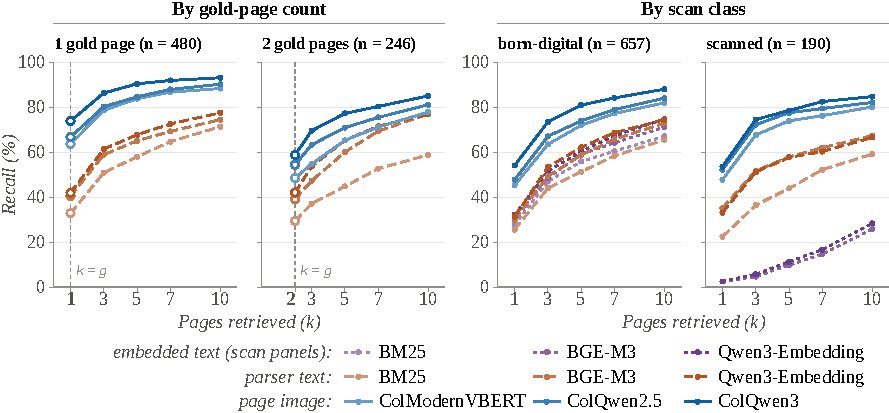
\includegraphics[width=0.95\textwidth]{appendix/figures/retrieval.pdf}
\caption{Page-level recall on MMLongBench-Doc by retrieval depth, split by gold-page count and by scan status.}
\label{fig:app_retrieval}
\end{figure*}

% GENERATED by ops/scripts/tables/ -- do not edit by hand, re-run the script.
% Numbers read from results/tables/longdocurl/ldu_selection_withholding.csv.
\definecolor{recwarm}{HTML}{D95926}
\definecolor{accteal}{HTML}{1BAF7A}
\begin{table}[t]
\centering
\small
\adjustbox{max width=\columnwidth}{%
\setlength{\tabcolsep}{3.5pt}%
\begin{tabular}{@{}l rr rr rr rr r@{}}
\toprule
 & \multicolumn{2}{c}{\textbf{Drop top}} & \multicolumn{2}{c}{\textbf{Drop bottom}} & \multicolumn{2}{c}{\textbf{Keep top}} & \multicolumn{2}{c}{\textbf{Keep bottom}} & \\
\cmidrule(lr){2-3}\cmidrule(lr){4-5}\cmidrule(lr){6-7}\cmidrule(lr){8-9}
\textbf{Source} & $-$ & $+$ & $-$ & $+$ & $-$ & $+$ & $-$ & $+$ & $n$ \\
\midrule
Text & \cellcolor{recwarm!51}48.1 & \cellcolor{accteal!2}2.1 & \cellcolor{recwarm!17}15.8 & \cellcolor{accteal!5}4.3 & \cellcolor{recwarm!20}19.3 & \cellcolor{accteal!4}3.7 & \cellcolor{recwarm!55}52.3 & \cellcolor{accteal!3}2.4 & 621 \\
Layout & \cellcolor{recwarm!38}36.5 & \cellcolor{accteal!2}1.6 & \cellcolor{recwarm!21}20.1 & \cellcolor{accteal!3}2.7 & \cellcolor{recwarm!25}23.4 & \cellcolor{accteal!2}2.3 & \cellcolor{recwarm!43}40.7 & \cellcolor{accteal!2}1.8 & 513 \\
Table & \cellcolor{recwarm!34}32.2 & \cellcolor{accteal!3}2.6 & \cellcolor{recwarm!17}15.9 & \cellcolor{accteal!4}3.9 & \cellcolor{recwarm!18}17.2 & \cellcolor{accteal!5}4.3 & \cellcolor{recwarm!35}33.0 & \cellcolor{accteal!2}1.7 & 233 \\
Figure & \cellcolor{recwarm!46}44.2 & \cellcolor{accteal!3}2.8 & \cellcolor{recwarm!24}22.7 & \cellcolor{accteal!5}4.4 & \cellcolor{recwarm!28}26.3 & \cellcolor{accteal!6}5.6 & \cellcolor{recwarm!51}48.2 & \cellcolor{accteal!3}2.4 & 251 \\
\midrule
\textbf{All} & \cellcolor{recwarm!45}43.2 & \cellcolor{accteal!2}2.0 & \cellcolor{recwarm!21}19.6 & \cellcolor{accteal!4}3.6 & \cellcolor{recwarm!23}22.2 & \cellcolor{accteal!4}3.5 & \cellcolor{recwarm!49}46.5 & \cellcolor{accteal!2}1.8 & 1{,}093 \\
\bottomrule
\end{tabular}%
}
\caption{LongDocURL verdict transitions after removing or retaining gold pages. Share (\%) of multi-page questions whose TLV verdict moves from correct to incorrect ($-$) or incorrect to correct ($+$) against the complete gold set; $n$ is the paired question count.}
\label{tab:app_ldu_coverage}
\end{table}
% {\footnotesize\raggedright
% Qwen3-VL-8B bf16, PaddleOCR-VL, medium resolution, no instruction, accuracy judge. Top and
% bottom are the highest- and lowest-ranked gold page under ColQwen3. Source rows overlap,
% so \textbf{All} pools each question once.\par}

% GENERATED by ops/scripts/tables/ -- do not edit by hand, re-run the script.
% Numbers read from results/tables/mmlongbench/robk_step_transitions.csv.
\definecolor{recwarm}{HTML}{D95926}
\definecolor{accteal}{HTML}{1BAF7A}
\begin{table}[t]
\centering
\small
\adjustbox{max width=\columnwidth}{%
\setlength{\tabcolsep}{3.5pt}%
\begin{tabular}{@{}ll rrrrrrr@{}}
\toprule
 & & \textbf{$+$3} & \textbf{$+$5} & \textbf{$+$7} & \textbf{$+$10} & \textbf{$+$13} & \textbf{$+$15} & \textbf{$+$18} \\
\midrule
\multicolumn{9}{@{}l}{\emph{Qwen3-VL-8B}} \\
\quad Single-hop & broken & \cellcolor{recwarm!47}12.4 & \cellcolor{recwarm!21}5.4 & \cellcolor{recwarm!21}5.4 & \cellcolor{recwarm!18}4.8 & \cellcolor{recwarm!25}6.6 & \cellcolor{recwarm!16}4.1 & \cellcolor{recwarm!15}3.8 \\
 & repaired & \cellcolor{accteal!33}8.7 & \cellcolor{accteal!21}5.4 & \cellcolor{accteal!12}3.1 & \cellcolor{accteal!16}4.2 & \cellcolor{accteal!22}5.7 & \cellcolor{accteal!12}3.2 & \cellcolor{accteal!9}2.3 \\
\quad Multi-hop & broken & \cellcolor{recwarm!55}14.4 & \cellcolor{recwarm!19}4.9 & \cellcolor{recwarm!26}6.8 & \cellcolor{recwarm!30}7.9 & \cellcolor{recwarm!20}5.2 & \cellcolor{recwarm!19}5.0 & -- \\
 & repaired & \cellcolor{accteal!21}5.6 & \cellcolor{accteal!25}6.5 & \cellcolor{accteal!29}7.7 & \cellcolor{accteal!16}4.3 & \cellcolor{accteal!16}4.1 & \cellcolor{accteal!23}5.9 & -- \\
\midrule
\multicolumn{9}{@{}l}{\emph{Gemma-3-12B}} \\
\quad Single-hop & broken & \cellcolor{recwarm!52}13.7 & \cellcolor{recwarm!27}7.1 & \cellcolor{recwarm!25}6.5 & \cellcolor{recwarm!30}7.9 & \cellcolor{recwarm!23}6.0 & \cellcolor{recwarm!27}7.1 & \cellcolor{recwarm!20}5.2 \\
 & repaired & \cellcolor{accteal!23}6.0 & \cellcolor{accteal!14}3.7 & \cellcolor{accteal!17}4.4 & \cellcolor{accteal!17}4.5 & \cellcolor{accteal!26}6.7 & \cellcolor{accteal!22}5.7 & \cellcolor{accteal!11}2.8 \\
\quad Multi-hop & broken & \cellcolor{recwarm!53}14.0 & \cellcolor{recwarm!27}7.0 & \cellcolor{recwarm!17}4.5 & \cellcolor{recwarm!20}5.3 & \cellcolor{recwarm!27}7.1 & \cellcolor{recwarm!19}5.0 & \cellcolor{recwarm!26}6.8 \\
 & repaired & \cellcolor{accteal!22}5.7 & \cellcolor{accteal!23}6.0 & \cellcolor{accteal!20}5.3 & \cellcolor{accteal!20}5.3 & \cellcolor{accteal!15}3.8 & \cellcolor{accteal!14}3.6 & \cellcolor{accteal!21}5.5 \\
\bottomrule
\end{tabular}%
}
\caption{Verdict transitions at each step of the distractor sweep. Share (\%) of questions whose TLV verdict moves from correct to incorrect (broken) or incorrect to correct (repaired) between one depth and the next, on MMLongBench-Doc; -- marks a step that has not completed.}
\label{tab:app_distractor_steps}
\end{table}
% {\footnotesize\raggedright
% Both reasoners at 4-bit with fp16 attention, medium resolution, no instruction, accuracy
% judge; non-gold pages ranked by ColQwen3. Each column is paired against the previous depth
% ($+3$ against the gold pages alone) on the questions that completed at both.\par}

% GENERATED by ops/scripts/tables/ -- do not edit by hand, re-run the script.
% Numbers read from results/tables/longdocurl/ldu_robk_curve.csv and
% ldu_robk_step_transitions.csv.
\definecolor{accteal}{HTML}{1BAF7A}
\definecolor{recwarm}{HTML}{D95926}
\begin{table}[t]
\centering
\small
\adjustbox{max width=\columnwidth}{%
\setlength{\tabcolsep}{3.5pt}%
\begin{tabular}{@{}ll rrrrrrrr@{}}
\toprule
 & & \textbf{$+$0} & \textbf{$+$3} & \textbf{$+$5} & \textbf{$+$7} & \textbf{$+$10} & \textbf{$+$13} & \textbf{$+$15} & \textbf{$+$18} \\
\midrule
Single-hop & accuracy & \cellcolor{accteal!60}77.2 & \cellcolor{accteal!13}68.5 & -- & -- & -- & -- & -- & -- \\
 & broken & -- & \cellcolor{recwarm!55}13.5 & -- & -- & -- & -- & -- & -- \\
 & repaired & -- & \cellcolor{accteal!20}4.8 & -- & -- & -- & -- & -- & -- \\
\midrule
Multi-hop & accuracy & \cellcolor{accteal!0}66.2 & -- & -- & -- & -- & -- & -- & -- \\
 & broken & -- & -- & -- & -- & -- & -- & -- & -- \\
 & repaired & -- & -- & -- & -- & -- & -- & -- & -- \\
\bottomrule
\end{tabular}%
}
\caption{LongDocURL accuracy and verdict transitions under added non-gold pages. Accuracy (\%) at TLV given every gold page plus the $k$ highest-ranked non-gold pages, with the share of questions broken or repaired against the previous depth; -- marks a depth that has not completed.}
\label{tab:app_ldu_distractor}
\end{table}
% {\footnotesize\raggedright
% Qwen3-VL-8B at 4-bit with fp16 attention, medium resolution, no instruction, accuracy judge,
% on the 1,000-question LongDocURL subset; non-gold pages ranked by ColQwen3. The sweep is
% still running: rerun the longdocurl report build and this script as its tags finish.\par}


% GENERATED by ops/scripts/tables/ -- do not edit by hand, re-run the script.
% Numbers read from results/tables/mmlongbench/reasoner_unified.csv and weight_footprint.csv.
\definecolor{accteal}{HTML}{1BAF7A}
\definecolor{recwarm}{HTML}{D95926}
\begin{table}[t]
\centering
\small
\adjustbox{max width=\columnwidth}{%
\setlength{\tabcolsep}{5pt}%
\begin{tabular}{@{}lrrrrr}
\toprule
\textbf{Reasoner} & \textbf{T} & \textbf{TL} & \textbf{TLV} & \textbf{V} & \textbf{GB} \\
\midrule
\multicolumn{6}{l}{\emph{Scale (Gemma-3, bf16)}} \\
\quad 4B & \cellcolor{accteal!8}22.1 & \cellcolor{accteal!16}30.5 & \cellcolor{accteal!26}39.5 & \cellcolor{accteal!20}33.6 & \cellcolor{recwarm!12}8.6 \\
\quad 12B & \cellcolor{accteal!16}30.5 & \cellcolor{accteal!23}36.9 & \cellcolor{accteal!34}48.1 & \cellcolor{accteal!28}41.6 & \cellcolor{recwarm!53}24.4 \\
\quad 27B & \cellcolor{accteal!19}32.8 & \cellcolor{accteal!26}40.0 & \cellcolor{accteal!38}52.0 & \cellcolor{accteal!31}44.6 & \cellcolor{recwarm!55}54.9 \\
\cmidrule(lr){1-6}
\multicolumn{6}{l}{\emph{Reasoning variant (Qwen3-VL-8B)}} \\
\quad Instruct & \cellcolor{accteal!18}31.9 & \cellcolor{accteal!24}38.4 & \cellcolor{accteal!38}52.4 & \cellcolor{accteal!32}45.5 & \cellcolor{recwarm!35}17.5 \\
\quad Thinking & \cellcolor{accteal!21}34.8 & \cellcolor{accteal!29}42.9 & \cellcolor{accteal!48}62.2 & \cellcolor{accteal!38}52.1 & \cellcolor{recwarm!35}17.5 \\
\bottomrule
\end{tabular}%
}
\caption{Accuracy for further reasoner configurations. Accuracy (\%) on answerable MMLongBench-Doc questions with gold pages; GB is the weight footprint.}
\label{tab:app_reasoner_configs}
\end{table}
% {\footnotesize\raggedright
% Medium resolution, no instruction, scored by the accuracy judge, so these levels sit about
% two to three points above the taxonomy-judged ones in the main text. The Gemma-3-12B and
% Instruct rows repeat the deployment table's, as the reference for the rows beside them.\par}

% GENERATED by ops/scripts/tables/ -- do not edit by hand, re-run the script.
% Numbers read from results/tables/mmlongbench/reasoner_hop_outcomes_gemma.csv.
\definecolor{accteal}{HTML}{1BAF7A}
\begin{table}[t]
\centering
\small
\adjustbox{max width=\columnwidth}{%
\setlength{\tabcolsep}{6pt}%
\begin{tabular}{@{}l rr r@{}}
\toprule
\textbf{Reasoner} & \textbf{Single-hop} & \textbf{Multi-hop} & \textbf{$\Delta$} \\
\midrule
Gemma-3-4B & \cellcolor{accteal!35}51.5 & \cellcolor{accteal!0}31.9 & 19.6 \\
Gemma-3-12B & \cellcolor{accteal!53}61.7 & \cellcolor{accteal!13}39.0 & 22.7 \\
Gemma-3-27B & \cellcolor{accteal!60}65.9 & \cellcolor{accteal!20}43.3 & 22.6 \\
\bottomrule
\end{tabular}%
}
\caption{Gemma-3 accuracy on single- and multi-hop questions by model size. Accuracy (\%) at TLV on answerable MMLongBench-Doc questions with gold pages; $\Delta$ is the multi-hop deficit.}
\label{tab:app_gemma_hops}
\end{table}
% {\footnotesize\raggedright
% bf16, medium resolution, no instruction, accuracy judge, on the 355 single-hop and 423
% multi-hop questions all three sizes completed. The counterpart of the Qwen3-VL scale figure
% in the main text.\par}

% GENERATED by ops/scripts/tables/ -- do not edit by hand, re-run the script.
% Numbers read from results/tables/mmlongbench/prompt_hop_outcomes.csv.
\definecolor{accteal}{HTML}{1BAF7A}
\definecolor{neutral}{HTML}{5B6B7F}
\begin{table}[t]
\centering
\small
\adjustbox{max width=\columnwidth}{%
\setlength{\tabcolsep}{5pt}%
\begin{tabular}{@{}l rr @{\hskip 10pt} rr@{}}
\toprule
 & \multicolumn{2}{c}{\textbf{Single-hop}} & \multicolumn{2}{c}{\textbf{Multi-hop}} \\
\cmidrule(lr){2-3}\cmidrule(l){4-5}
\textbf{Prompt mode} & \textbf{Acc.} & \textbf{Ref.} & \textbf{Acc.} & \textbf{Ref.} \\
\midrule
\texttt{none} & \cellcolor{accteal!60}\textbf{66.4} & \cellcolor{neutral!2}1.4 & \cellcolor{accteal!19}44.9 & \cellcolor{neutral!3}1.5 \\
\texttt{grounded} & \cellcolor{accteal!46}59.2 & \cellcolor{neutral!1}0.6 & \cellcolor{accteal!7}38.5 & \cellcolor{neutral!0}0.5 \\
\texttt{abstain} & \cellcolor{accteal!36}53.7 & \cellcolor{neutral!47}22.0 & \cellcolor{accteal!0}34.7 & \cellcolor{neutral!60}28.1 \\
\texttt{abstain\_balanced} & \cellcolor{accteal!39}55.1 & \cellcolor{neutral!37}17.6 & \cellcolor{accteal!2}35.7 & \cellcolor{neutral!51}23.7 \\
\texttt{cot} & \cellcolor{accteal!55}63.6 & \cellcolor{neutral!0}0.3 & \cellcolor{accteal!25}\textbf{48.0} & \cellcolor{neutral!3}1.5 \\
\texttt{extract\_cot} & \cellcolor{accteal!46}59.2 & \cellcolor{neutral!1}0.8 & \cellcolor{accteal!19}44.6 & \cellcolor{neutral!4}2.3 \\
\texttt{abstain\_cot} & \cellcolor{accteal!54}63.1 & \cellcolor{neutral!35}16.3 & \cellcolor{accteal!17}43.9 & \cellcolor{neutral!47}21.9 \\
\bottomrule
\end{tabular}%
}
\caption{Prompt-mode results on single- and multi-hop questions. Accuracy and refusal (\%) at TLV on answerable MMLongBench-Doc questions with gold pages.}
\label{tab:app_prompt_hops}
\end{table}
% {\footnotesize\raggedright
% Qwen3-VL-8B bf16, medium resolution, accuracy judge, on the 363 single-hop and 392 multi-hop
% questions every prompt mode completed. Refusal counts refusals the judge did not credit.\par}

% GENERATED by ops/scripts/tables/ -- do not edit by hand, re-run the script.
% Numbers read from results/tables/analysis/faithfulness_answerable_accuracy_source.csv and
% error_profile_prompt_unanswerable.csv (results.errcat.jsonl).
\definecolor{accteal}{HTML}{1BAF7A}
\definecolor{neutral}{HTML}{5B6B7F}
\begin{table*}[t]
\centering
\small
\adjustbox{max width=\textwidth}{%
\setlength{\tabcolsep}{5pt}%
\begin{tabular}{@{}l rrrrrr @{\hskip 12pt} rrrrrr @{\hskip 12pt} r@{}}
\toprule
 & \multicolumn{6}{c}{\textbf{Answerable accuracy}} & \multicolumn{6}{c}{\textbf{Answerable refusal}} & \textbf{Unans.} \\
\cmidrule(r){2-7}\cmidrule(lr){8-13}\cmidrule(l){14-14}
\textbf{Prompt mode} & \textbf{Text} & \textbf{Layout} & \textbf{Table} & \textbf{Chart} & \textbf{Figure} & \textbf{All} & \textbf{Text} & \textbf{Layout} & \textbf{Table} & \textbf{Chart} & \textbf{Figure} & \textbf{All} & \textbf{refusal} \\
\midrule
\texttt{none} & \cellcolor{accteal!59}\textbf{51.0} & \cellcolor{accteal!55}49.2 & \cellcolor{accteal!44}44.7 & \cellcolor{accteal!39}42.7 & \cellcolor{accteal!38}42.4 & \cellcolor{accteal!55}49.5 & \cellcolor{neutral!12}7.3 & \cellcolor{neutral!1}0.8 & \cellcolor{neutral!11}6.7 & \cellcolor{neutral!12}7.3 & \cellcolor{neutral!13}7.6 & \cellcolor{neutral!10}6.2 & \cellcolor{accteal!13}45.5 \\
\texttt{grounded} & \cellcolor{accteal!54}49.0 & \cellcolor{accteal!40}43.2 & \cellcolor{accteal!29}38.5 & \cellcolor{accteal!12}31.5 & \cellcolor{accteal!34}40.7 & \cellcolor{accteal!42}43.7 & \cellcolor{neutral!12}7.0 & \cellcolor{neutral!0}0.0 & \cellcolor{neutral!12}7.2 & \cellcolor{neutral!9}5.1 & \cellcolor{neutral!12}7.2 & \cellcolor{neutral!10}6.0 & \cellcolor{accteal!0}37.3 \\
\texttt{abstain} & \cellcolor{accteal!42}43.7 & \cellcolor{accteal!36}41.5 & \cellcolor{accteal!29}38.5 & \cellcolor{accteal!0}26.4 & \cellcolor{accteal!18}34.1 & \cellcolor{accteal!33}40.0 & \cellcolor{neutral!41}\textbf{24.1} & \cellcolor{neutral!33}\textbf{19.5} & \cellcolor{neutral!51}\textbf{30.3} & \cellcolor{neutral!43}\textbf{25.3} & \cellcolor{neutral!60}\textbf{35.5} & \cellcolor{neutral!47}\textbf{27.7} & \cellcolor{accteal!60}\textbf{74.6} \\
\texttt{abstain\_balanced} & \cellcolor{accteal!46}45.5 & \cellcolor{accteal!36}41.5 & \cellcolor{accteal!22}35.6 & \cellcolor{accteal!4}28.1 & \cellcolor{accteal!22}35.5 & \cellcolor{accteal!35}40.9 & \cellcolor{neutral!32}19.2 & \cellcolor{neutral!31}18.6 & \cellcolor{neutral!43}25.5 & \cellcolor{neutral!31}18.5 & \cellcolor{neutral!53}31.4 & \cellcolor{neutral!39}23.2 & \cellcolor{accteal!51}68.9 \\
\texttt{cot} & \cellcolor{accteal!59}\textbf{51.0} & \cellcolor{accteal!55}49.2 & \cellcolor{accteal!60}\textbf{51.4} & \cellcolor{accteal!41}\textbf{43.3} & \cellcolor{accteal!42}\textbf{43.8} & \cellcolor{accteal!57}\textbf{50.2} & \cellcolor{neutral!13}7.7 & \cellcolor{neutral!6}3.4 & \cellcolor{neutral!12}7.2 & \cellcolor{neutral!16}9.6 & \cellcolor{neutral!12}6.9 & \cellcolor{neutral!11}6.6 & \cellcolor{accteal!9}43.0 \\
\texttt{extract\_cot} & \cellcolor{accteal!52}48.2 & \cellcolor{accteal!60}\textbf{51.3} & \cellcolor{accteal!54}49.0 & \cellcolor{accteal!24}36.6 & \cellcolor{accteal!41}43.3 & \cellcolor{accteal!51}47.5 & \cellcolor{neutral!17}9.9 & \cellcolor{neutral!4}2.6 & \cellcolor{neutral!16}9.6 & \cellcolor{neutral!11}6.3 & \cellcolor{neutral!19}11.1 & \cellcolor{neutral!15}8.8 & \cellcolor{accteal!17}47.7 \\
\bottomrule
\end{tabular}%
}
\caption{Prompt-mode results at TLV. Rates (\%) on MMLongBench-Doc: accuracy and refusal on answerable questions with gold pages, by evidence source, and refusal on unanswerable questions with BM25's top three pages, where refusing is correct.}
\label{tab:app_prompt_results}
\end{table*}
% {\footnotesize\raggedright
% Qwen3-VL-8B bf16, medium resolution, under the error-taxonomy judge. Answerable refusal counts
% refusals the judge did not credit. Unanswerable refusal is 100 minus the pool's wrong
% responses, since a refusal is the only correct response there; that pool carries no
% evidence-source labels, so it has no source breakdown.\par}


%% ---------------------------------------------------------------------------
\subsection{Representation}
\label{app:results_representation}

\paragraph{Parsers by Evidence Source.}
Table~\ref{tab:app_parser_sources} breaks the parser comparison of Figure~\ref{fig:fidelity} down by evidence source. The page image helps most where text extraction loses the evidence: chart and figure questions gain 13 to 26 points on born-digital documents under every text source, while table questions change by under 6 points and lose slightly under three of the four. On scanned documents embedded text answers almost nothing, and the image recovers 45 points or more for every source.

\paragraph{Resolution by Evidence Source.}
Table~\ref{tab:app_resolution_sources} extends the resolution sweep to all evidence sources. From \texttt{low} to \texttt{high}, \textbf{V} gains 12.4 points overall and 17.1 on tables, against 5.5 and 0.0 for \textbf{TLV}. Chart questions are the exception: they gain about 10 points under \textbf{TLV} as well, and parser text adds nothing to them at \texttt{med} or \texttt{high}.

\paragraph{LongDocURL by Question Type.}
Table~\ref{tab:app_ldu_types} splits the LongDocURL results of Table~\ref{tab:ldu_rungs} by question type. Accuracy varies far more across question types than across representations: \texttt{summary2tab} stays below 20\% under every representation, while \texttt{extract} never falls below 74\%. Parser text alone is the best representation for two of the locating types, and \textbf{V} is weakest on \texttt{calculate} and \texttt{compare}, which depend on exact values.

%% ---------------------------------------------------------------------------
\subsection{Selection}
\label{app:results_selection}

\paragraph{Retrieval Recall.}
Figure~\ref{fig:app_retrieval} compares three text and three visual retrievers. Visual retrievers lead at every depth, and ColQwen3 is the strongest, which is why it orders pages in the selection experiments. Text retrieval over the embedded text layer collapses on scanned documents, and ranking parser text instead recovers much of the gap. Even ColQwen3 leaves gold pages outside the top ten, more often for questions with two gold pages.

\paragraph{Coverage on LongDocURL.}
Table~\ref{tab:app_ldu_coverage} repeats the coverage experiment of Figure~\ref{fig:coverage} on LongDocURL. Omission again breaks far more answers than it repairs. Unlike on MMLongBench-Doc, retrieval rank is informative here: removing the highest-ranked gold page breaks 43.2\% of answers, against 19.6\% for the lowest-ranked page.

\paragraph{Distractor Transitions by Step.}
Table~\ref{tab:app_distractor_steps} gives the paired transitions behind Figures~\ref{fig:distractor_k} and~\ref{fig:distractor_transfer_family}, comparing each depth with the one before it. The first three added pages break 12 to 14\% of answers for both reasoners and both question groups, well above any later step (at most 7.9\%). Every step also repairs answers, at 2 to 9\%, so the accuracy curve is the net of two opposing movements. After the first step the two roughly cancel for Qwen3-VL-8B, while broken answers continue to outnumber repaired ones at most steps for Gemma-3-12B on single-hop questions.

\paragraph{Distractors on LongDocURL.}
Table~\ref{tab:app_ldu_distractor} repeats the distractor sweep on LongDocURL with Qwen3-VL-8B. This experiment is still running, and the table reports the depths completed so far. On single-hop questions the first three added pages lower accuracy from 77.2\% to 68.5\%, breaking 13.5\% of answers and repairing 4.8\%, close to the first step on MMLongBench-Doc.

%% ---------------------------------------------------------------------------
\subsection{Reasoning}
\label{app:results_reasoning}

\paragraph{Further Reasoner Configurations.}
Table~\ref{tab:app_reasoner_configs} adds two comparisons to Table~\ref{tab:deploy_reasoner}. Gemma-3 improves with scale at every representation, as Qwen3-VL does, reaching 52.0\% at \textbf{TLV} with 27B. The Thinking variant of Qwen3-VL-8B reaches 62.2\% at \textbf{TLV}, 9.8 points above the Instruct model at the same weight footprint and above the 32B Instruct model.

\paragraph{Gemma-3 Scale by Hop.}
Table~\ref{tab:app_gemma_hops} repeats the scale comparison of Figure~\ref{fig:integration_scale} for Gemma-3. Multi-hop accuracy rises from 31.9\% at 4B to 43.3\% at 27B, and single-hop accuracy rises alongside it, so the gap between them does not narrow (19.6 points at 4B, 22.6 at 27B), as with Qwen3-VL.

\paragraph{Prompt Modes by Hop.}
Table~\ref{tab:app_prompt_hops} splits the prompt modes by evidence structure. The near-zero overall effect of \texttt{cot} reported in \S\ref{sec:findings_reasoning} hides two opposite ones: it raises multi-hop accuracy by 3.1 points and lowers single-hop accuracy by 2.8. \texttt{abstain} costs accuracy on both, and multi-hop questions are refused more often (28.1\% against 22.0\%). \texttt{abstain\_cot} recovers most of that loss on both.

\paragraph{Prompt Modes by Evidence Source.}
Table~\ref{tab:app_prompt_results} reports six prompt modes by evidence source under the taxonomy rubric. Its refusal rates are higher than those of Table~\ref{tab:app_prompt_hops} and Figure~\ref{fig:reasoning_abstain_cot}, which use the accuracy rubric, but the pattern is the same: \texttt{abstain} raises unanswerable refusal from 45.5\% to 74.6\% and answerable refusal from 6.2\% to 27.7\%, with figure and table questions refused most. Adding a sentence against declining supported questions (\texttt{abstain\_balanced}) recovers little, and \texttt{grounded} alone lowers accuracy without improving refusal.

%% ---------------------------------------------------------------------------
\subsection{Error Analysis}
\label{app:results_errors}

\begin{figure*}[t]
\centering
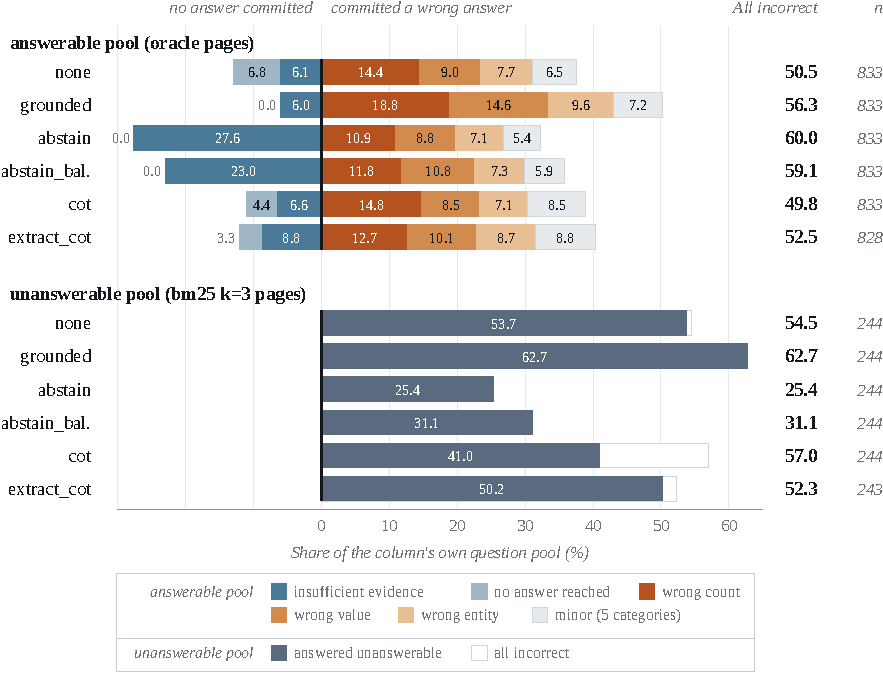
\includegraphics[width=0.72\textwidth]{appendix/figures/error_profile.pdf}
\caption{Error categories by prompt mode on answerable and unanswerable questions.}
\label{fig:app_error_profile}
\end{figure*}

\begin{figure*}[t]
\centering
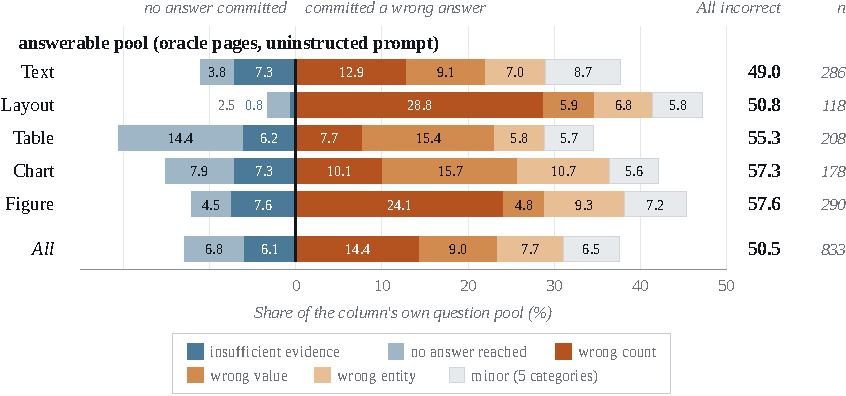
\includegraphics[width=0.69\textwidth]{appendix/figures/error_sources.pdf}
\caption{Error categories by evidence source on answerable questions with no instruction.}
\label{fig:app_error_sources}
\end{figure*}

The taxonomy rubric assigns each incorrect response one error category (Table~\ref{tab:app_error_taxonomy}). Figures~\ref{fig:app_error_profile} and~\ref{fig:app_error_sources} show the share of each category, with responses that commit to no answer on the left and wrong answers on the right.

\paragraph{By Prompt Mode.}
The abstention instructions change the kind of error more than its amount (Figure~\ref{fig:app_error_profile}). Under \texttt{abstain}, refusals on answerable questions rise from 6.1\% to 27.6\% while every wrong-answer category shrinks, and answers to unanswerable questions fall from 53.7\% to 25.4\%. \texttt{grounded} moves in the opposite direction, removing unfinished responses but adding wrong values and counts.

\paragraph{By Evidence Source.}
Wrong counts dominate layout and figure questions, at 28.8\% and 24.1\% (Figure~\ref{fig:app_error_sources}). Table and chart questions fail mainly on values, and table questions most often end without stating an answer.


\clearpage
% The page of full-width figures before this one leaves LaTeX with a short height for the
% next column, which would push the first example into the second column. Reset it.
\makeatletter\global\@colroom\@colht\global\vsize\@colht\makeatother
\section{Worked Examples}
\label{app:examples}

% Worked-example boxes. Macro namespace: \wx* only.
\definecolor{wxright}{HTML}{1BAF7A}
\definecolor{wxwrong}{HTML}{D95926}
\definecolor{wxhold}{HTML}{C8891B}
\definecolor{wxrule}{HTML}{BFBFBF}
\definecolor{wxtitle}{HTML}{EFEFEF}
\newcommand{\wxR}{\textcolor{wxright}{$\checkmark$}}
\newcommand{\wxW}{\textcolor{wxwrong}{$\times$}}
\newcommand{\wxA}{\textcolor{wxhold}{$\circ$}}
\newtcolorbox{wxbox}[3]{%
  breakable, enhanced, sharp corners, boxrule=0.4pt,
  colback=white, colframe=wxrule,
  left=4pt, right=4pt, top=3pt, bottom=3pt,
  toptitle=1pt, bottomtitle=1pt,
  colbacktitle=wxtitle, coltitle=black, titlerule=0pt,
  fonttitle=\footnotesize, halign title=flush left,
  title={\textbf{#1}\hspace{0.6em}\textbf{#2}\hfill\texttt{\scriptsize #3}},
}
\newcommand{\wxmeta}[1]{{\scriptsize\textcolor{black!62}{#1}\par}\vspace{1.5pt}}
\newcommand{\wxq}[1]{{\footnotesize\textbf{Q}\hspace{0.5em}#1\par}}
\newcommand{\wxgold}[1]{{\footnotesize\textbf{Gold}\hspace{0.5em}#1\par}}
\newcommand{\wxsep}{\vspace{2.5pt}{\color{wxrule}\hrule height 0.4pt}\vspace{2.5pt}}
\newcommand{\wxrow}[3]{%
  \par\vspace{1.5pt}%
  \noindent%
  \parbox[t]{0.300\linewidth}{\footnotesize\raggedright #1}%
  \hspace{1pt}%
  \parbox[t]{0.045\linewidth}{\footnotesize #2}%
  \hspace{1pt}%
  \parbox[t]{0.620\linewidth}{\footnotesize\raggedright #3}\par}
\newcommand{\wxnote}[1]{{\footnotesize #1\par}}
\newcommand{\wxsnip}[1]{%
  \par\vspace{2pt}\noindent\hspace{0.02\linewidth}%
  \parbox{0.96\linewidth}{\scriptsize\ttfamily\raggedright\sloppy #1}\par\vspace{2pt}}
\newcommand{\wxread}[1]{\wxsep{\footnotesize\textit{#1}\par}}

This appendix shows individual questions behind the rates of \S\ref{sec:findings}, at least one for each failure mechanism of \S\ref{sec:attribution_framework}. Each box gives the question, the gold answer, and the reasoner's output under every condition shown, marked \wxR{} correct, \wxW{} incorrect or \wxA{} abstained. The reasoner is Qwen3-VL-8B at \textbf{TLV} with no instruction unless a row says otherwise, and verdicts follow the accuracy rubric. Page numbers are zero-based indices into the document. None of these questions is one of the six in Figure~\ref{fig:mechanism_examples}.

%% ---------------------------------------------------------------------------
\subsection{Representation}
\label{app:ex_representation}

\begin{wxbox}{R1}{Modality ceiling}{mmlongbench:000014}
\wxmeta{Presentation deck (Tutorial/Workshop), born-digital. Gold page 13, a single chart. Evidence source: chart.}
\wxq{According to the chart on page 14 how much time was spent with family and friends in 2010?}
\wxgold{21\%}
\wxsep
\wxnote{The page is one chart, and the parser has nothing to transcribe. PaddleOCR-VL emits only a placeholder:}
\wxsnip{<div style="text-align: center;"><img src="[\ldots]" alt="Image" width="52\%" /></div>}
\wxsep
\wxrow{T}{\wxA}{``The document does not provide any evidence or chart on page 14, so it is not possible to determine how much time was spent with family and friends in 2010 [\ldots]''}
\wxrow{TL}{\wxA}{``[\ldots] The image referenced (on page 14) is not described or transcribed, so its content cannot be interpreted. [\ldots]''}
\wxrow{V}{\wxR}{``According to the chart on page 14, in 2010, 21\% of weekend time was spent with family and friends.''}
\wxrow{TLV}{\wxR}{``According to the chart on page 14, in 2010, 21\% of weekend time was spent with family and friends.''}
\wxread{The gold page reaches every representation, so nothing is missing from the context. The value lives in the chart's geometry and no text channel carries it, so both text representations decline instead of guessing, which is the refusal pattern of Table~\ref{tab:abstention_rungs}.}
\end{wxbox}

\begin{wxbox}{R2}{Conversion fidelity: parser}{mmlongbench:000513}
\wxmeta{Guidebook, born-digital. Gold page 9, a numbered list of market names with a code beside each. Evidence source: text and table.}
\wxq{How many geographic market names are listed under Los Angeles area?}
\wxgold{13}
\wxsep
\wxnote{The list runs from item 14 to item 26. The three parsers keep its text and differ in what they do with the code column:}
\wxsnip{PaddleOCR-VL: California 14-26 \textbar{} 14. San Fernando Valley (West) CA14 \textbar{} [\ldots] \textbar{} 26. Santa Ana CA26 \\[1.5pt] MinerU 2.5: 14. San Fernando Valley (West) \textbar{} [\ldots] \textbar{} 26. Santa AnaEPS \textbar{} Code \textbar{} 4.14 \textbar{} [\ldots] \textbar{} 4.26 \\[1.5pt] Unlimited-OCR: <table><tr><td>14.</td><td>San Fernando Valley (West)</td><td>CA14</td></tr> [\ldots]}
\wxsep
\wxrow{T}{\wxR}{``The document lists \textbf{13} geographic market names under the Los Angeles area. [\ldots]''}
\wxrow{TL, PaddleOCR-VL}{\wxW}{``26 The document lists 26 geographic market names under the `Los Angeles Area' section, ranging from CA14 to CA26.''}
\wxrow{TL, MinerU 2.5}{\wxW}{``26 The document lists 26 geographic market names [\ldots] ranging from `San Fernando Valley (West)' (item 14) to `Santa Ana' (item 26).''}
\wxrow{TL, Unlimited-OCR}{\wxR}{``There are \textbf{13} geographic market names listed under the Los Angeles area. The list includes entries numbered 14 through 26 [\ldots]''}
\wxrow{TLV, PaddleOCR-VL}{\wxR}{``[\ldots] there are \textbf{13} geographic market names listed under the Los Angeles area. [\ldots] codes from 14 to 26. Counting these entries [\ldots]''}
\wxread{Every parser returns all thirteen names, yet two flatten the list so that its last label reads as its length. The parser that keeps the rows as a table gives the right count, as does the same flattened parse once the page image accompanies it: the image is the redundant channel that absorbs the conversion error.}
\end{wxbox}

\begin{wxbox}{R3}{Conversion fidelity: resolution}{mmlongbench:000065}
\wxmeta{Academic paper, born-digital. Gold page 6, a results table with one row per model and temperature. Evidence source: text and table.}
\wxq{From the paper, which temperature gives ChatGPT the highest alignment score?}
\wxgold{0.1}
\wxsep
\wxrow{V, \texttt{low}}{\wxW}{``[\ldots] the temperature that gives ChatGPT the highest alignment score is \textbf{0.5}.''}
\wxrow{V, \texttt{med}}{\wxW}{``[\ldots] is \textbf{0.5}. [\ldots] Table 3 lists three ChatGPT models: ChatGPT (0.5), ChatGPT (0.1), and ChatGPT (0.9) [\ldots]''}
\wxrow{V, \texttt{high}}{\wxR}{``[\ldots] the temperature that gives ChatGPT the highest alignment score is \textbf{0.1}.''}
\wxrow{TLV, \texttt{low}}{\wxR}{``[\ldots] ChatGPT (0.1): 85.9, ChatGPT (0.5): 84.5, ChatGPT (0.9): 84.1. [\ldots] \textbf{85.9} is the highest alignment score, which corresponds to [\ldots] \textbf{0.1}.''}
\wxread{The image alone finds the right table at every resolution but only reads its small digits correctly at \texttt{high}. With parser text the values are available as characters, so the lowest resolution already suffices, as in the table rows of Table~\ref{tab:app_resolution_sources}.}
\end{wxbox}

%% ---------------------------------------------------------------------------
\subsection{Selection}
\label{app:ex_selection}

\begin{wxbox}{S1}{Evidence coverage}{mmlongbench:000082}
\wxmeta{Survey paper (Academic paper), born-digital. Gold pages 8 and 9: the sentence that answers the question starts on the last line of page 8 and finishes on page 9. \texttt{drop\_top} leaves page 8 and \texttt{drop\_bottom} page 9. Evidence source: text.}
\wxq{Which method integrates knowledge into white-box models via directive fine-tuning?}
\wxgold{PKG}
\wxsep
\wxrow{gold pages}{\wxR}{``[\ldots] the method that integrates knowledge into white-box models via directive fine-tuning is \textbf{PKG}. [\ldots] `PKG introduces an innovative method for integrating knowledge into white-box models via directive fine-tuning [75].' [\ldots]''}
\wxrow{\texttt{drop\_top}}{\wxW}{``[\ldots] the method that integrates knowledge into white-box models via directive fine-tuning is \textbf{Fine-tuning Embedding Model}. [\ldots]''}
\wxrow{\texttt{drop\_bottom}}{\wxW}{``The method that integrates knowledge into white-box models via directive fine-tuning is \textbf{directive fine-tuning}. The document explicitly states: `introduces an innovative method for integrating knowledge into white-box models via directive fine-tuning [75].' [\ldots]''}
\wxread{Page 8 ends on the method's name and page 9 opens with what it does, so neither page holds the answer. With one of them withheld the reasoner does not decline: it names a nearby section heading, or repeats the question's own phrase. Both removals break the answer, so retrieval rank does not identify a page that can safely be omitted.}
\end{wxbox}

\begin{wxbox}{S2}{Distractor exposure: broken}{mmlongbench:000078}
\wxmeta{Survey paper (Academic paper), born-digital, multi-hop. Gold pages 5 (a table of methods) and 16 (the reference list). $+3$ adds pages 0, 6 and 7; page 0 is the survey's own title page. 4-bit weights.}
\wxq{What is the paper's full title that proposes the method that has a retrieval granularity of phrase?}
\wxgold{Copy is all you need.}
\wxsep
\wxrow{gold only}{\wxR}{``[\ldots] the method with a retrieval granularity of ``Phrase'' is \textbf{CoG [29]}. [\ldots] the full title of the paper proposing the CoG method is: \textbf{``Copy is all you need''}. This is found in the References section [\ldots]''}
\wxrow{$+3$}{\wxW}{``[\ldots] the paper's full title is \textbf{Retrieval-Augmented Generation for Large Language Models: A Survey}. This is explicitly stated in the title section of the document [\ldots]''}
\wxrow{$+5$ to $+18$}{\wxW}{The same answer at every completed depth.}
\wxread{Both gold pages are still present and nothing in them changed. The added title page is a plausible partial match for ``the paper's full title'', and the reasoner takes it instead of following the table entry to its reference. Coverage is complete; the failure is in using the evidence amid competing context.}
\end{wxbox}

\begin{wxbox}{S3}{Distractor exposure: repaired}{mmlongbench:000243}
\wxmeta{Rezoning study (Research report), born-digital, single-hop. Gold page 7, which carries a table of residential capacity by borough. $+3$ adds pages 4, 8 and 12, the surrounding discussion. 4-bit weights.}
\wxq{What is the residential capacity of Staten Island from 2003 to 2007? Give me an integer.}
\wxgold{435000000}
\wxsep
\wxrow{gold only}{\wxW}{``80000''}
\wxrow{$+3$}{\wxR}{``435000000''}
\wxrow{$+10$}{\wxR}{``435000000''}
\wxrow{$+13$}{\wxW}{``5980000''}
\wxrow{$+18$}{\wxR}{``435000000''}
\wxread{The table holding the answer is supplied in every row. The reasoner misreads it in isolation and reads it correctly once neighbouring pages of the same section are present, then fails again at one deeper setting. Added pages therefore both repair and break answers on the same question, the two-way movement behind the transitions of Figure~\ref{fig:distractor_k}.}
\end{wxbox}

\paragraph{Distractors on LongDocURL.}
Table~\ref{tab:app_ldu_distractor} repeats the distractor sweep on LongDocURL with Qwen3-VL-8B. This experiment is still running, and the table reports the depths completed so far. On single-hop questions the first three added pages lower accuracy from 77.2\% to 68.5\%, breaking 13.5\% of answers and repairing 4.8\%, close to the first step on MMLongBench-Doc.

%% ---------------------------------------------------------------------------
\subsection{Reasoning}
\label{app:ex_reasoning}

\begin{wxbox}{N1}{Evidence integration}{mmlongbench:001015}
\wxmeta{Annual report (Financial report), born-digital, multi-hop. Gold pages 35 (the income statement) and 39 (the cash flow statement). Rows are Qwen3-VL sizes. Evidence source: table.}
\wxq{what is EBITDA for costco in FY2021?}
\wxgold{8489}
\wxsep
\wxrow{2B}{\wxW}{``[\ldots] EBITDA for Costco in FY2021 is \$6,708 million. This is found in the [\ldots] row labeled `Operating income' [\ldots]''}
\wxrow{4B}{\wxW}{``The EBITDA for Costco in FY2021 is \$6,708 million. [\ldots] EBITDA [\ldots] is typically calculated as Operating Income plus Depreciation and Amortization, but in this document, the `Operating income' row is presented as the direct measure of EBITDA [\ldots]''}
\wxrow{8B}{\wxW}{``[\ldots] Operating Income + Depreciation and Amortization + Interest Expense + Provision for Income Taxes = \$6,708 + \$1,781 + \$(171) + \$1,601 = \textbf{\$8,469 million}''}
\wxrow{32B}{\wxR}{``[\ldots] From the Consolidated Statements of Income: Operating Income = \$6,708 million. From the Consolidated Statements of Cash Flows: Depreciation and Amortization = \$1,781 million. [\ldots] \$6,708 + \$1,781 = \textbf{\$8,489 million}''}
\wxread{Every model receives the same two statements. The two smallest stop at operating income on the first page, one of them after stating the formula that needs the second. The 8B reaches the cash flow statement but adds lines that operating income already excludes, and only the largest joins the two operands. The evidence was sufficient throughout; what scales is the ability to combine it.}
\end{wxbox}

\begin{wxbox}{N2}{Response calibration: answerable}{mmlongbench:000418}
\wxmeta{E-commerce market deck (Research report), scanned, multi-hop. Gold pages 11 and 14, one bar chart on each. Evidence source: chart.}
\wxq{How many people in India were using a debit card when the e-commerce sales reached 11 billion?}
\wxgold{399 million}
\wxsep
\wxrow{\texttt{none}}{\wxR}{``[\ldots] when e-commerce sales reached \$11 billion (in 2014), the number of debit card users in India was \textbf{399 million}. [\ldots]''}
\wxrow{\texttt{cot}}{\wxR}{``Step 1: [\ldots] the \$11 billion mark is shown for the year 2014. Step 2: [\ldots] the bar chart titled `Number of Debit Card users in India (In millions)' shows the value for 2014 as 399 million. [\ldots] Answer: 399 million''}
\wxrow{\texttt{abstain}}{\wxA}{``Not answerable''}
\wxrow{\texttt{abstain\_cot}}{\wxR}{``Step 1: [\ldots] e-commerce sales were \$11 billion in 2014. Step 2: [\ldots] For 2014, the number is 399 million. [\ldots] Answer: 399 million''}
\wxread{The answer is on neither page alone: one chart gives the year, the other the count for that year. Under \texttt{abstain} the reasoner refuses a question it answers correctly with no instruction, a false refusal. Asking it to reason before deciding makes it locate both values first, and the refusal disappears.}
\end{wxbox}

\begin{wxbox}{N3}{Response calibration: unanswerable}{mmlongbench:000047}
\wxmeta{Data-leadership talk (Tutorial/Workshop), scanned, unanswerable. BM25's top three pages (0, 1, 2) are supplied; the document mentions no video.}
\wxq{Which Youtube does the slides use to show the consequce of having a weak data leadership?}
\wxgold{Not answerable}
\wxsep
\wxrow{\texttt{none}}{\wxW}{``The slides use a YouTube clip from the TV show \textit{Breaking Bad} to illustrate the consequence of having weak data leadership [\ldots] as symbolized by the character Walter White hoarding money [\ldots]''}
\wxrow{\texttt{cot}}{\wxR}{``[\ldots] Step 4: However, the document evidence does not mention any YouTube or reference any video content. The image is a still image, not a YouTube video. [\ldots] Answer: Not specified in the document.''}
\wxrow{\texttt{abstain}}{\wxR}{``Not answerable''}
\wxrow{\texttt{abstain\_cot}}{\wxR}{``[\ldots] Step 3: The document does not mention YouTube at all. [\ldots] Answer: Not answerable''}
\wxread{One supplied page shows a man holding stacks of money, and with no instruction the reasoner builds a show, a character and an interpretation out of it. Each of the other prompts leads it to check the premise against the pages and decline, which is the correct response here.}
\end{wxbox}
z

\clearpage
\input{appendix/appendix_D}

\end{document}